\documentclass[letter, 12pt]{turabian-thesis}
\setlength{\skip\footins}{1.2pc plus 5pt minus 10pt}
\usepackage[english]{babel}
\usepackage[utf8]{inputenc}
\usepackage{csquotes}
\usepackage{biblatex-chicago}
\usepackage{paralist}
\usepackage{amsthm}
\usepackage{amsmath}
\usepackage{ragged2e}

\usepackage{bm}
\usepackage{amssymb}
\usepackage{physics}
\usepackage{gensymb} 
\usepackage{csquotes}
\usepackage{enumitem}
\usepackage{comment}
\usepackage{mathtools}
\usepackage{siunitx}
\usepackage[acronym, nopostdot, nonumberlist, section]{glossaries}
\usepackage{glossary-mcols}
\usepackage{etoolbox}
\usepackage{graphicx} % Required for including images
\usepackage{tikz}
\usepackage{caption}
\usepackage{parskip}
\usepackage{bigfoot}

\usepackage[inline]{showlabels}


\thispagestyle{empty}
\makeatletter
\patchcmd{\chapter}{\if@openright\cleardoublepage\else\clearpage\fi}{}{}{}
\makeatother

\setcounter{secnumdepth}{5}
\newglossarystyle{mylong}{% 
\glossarystyle{long}% base this style on the list style 
\renewcommand{\glsgroupskip}{}% make nothing happen between groups 
}
\glossarystyle{mylong}


\newcommand{\du}[2]{\mathbf{\SI[inter-unit-product={}\cdot{}]{#1}{#2}}}

\makeatletter 
\newcommand{\pp@spage}{}
\makeatother

\theoremstyle{hypothesis}
\newtheorem*{hypothesis}{Partitioning Criterion}
\newcommand\myeq{\stackrel{\mathclap{\scriptsize\mbox{def}}}{=}}
\newcommand{\uvb}[1]{\vb{\hat{{#1}}}}
\newcommand{\uvbp}[1]{\uvb{#1}\bm{+}}
\newcommand{\uvbm}[1]{\uvb{#1}\bm{-}}
\newcommand{\uvbpm}[1]{\uvb{#1}\bm{\pm}}
\newcommand{\dotsize}{2pt}
\makeatletter 
\def\footnoterule{\kern-6\p@ % you can put other values to increase vertical space between rule and notes (just try out); difference between the values after "kern" is the width of the rule!
\hrule \@width 2in \kern 5.7\p@} % the in value is the length of the footnoterule
% footnotemark

\renewcommand{\@makefntext}[1]{%
\if@optraggedright
\raggedright%
\fi
\setlength{\parindent}{\footnotemargin}%
\textsuperscript{\@thefnmark}#1%
}

\addtolength{\skip\footins}{2pt} % vertical space between rule and main text
\setlength{\footnotesep}{12pt} % vertical space between footnotes
\let\origfootnote\footnote % font size of footnotes; changes \footnotesize command only inside footnotes!
\setlength{\footnotemargin}{0in}
\renewcommand{\footnote}[1]{%
\noindent % here there is scriptsize in footnotes (example) 
\origfootnote{#1}} 

\makeatother




\usepackage{url}



\let\URL\url
\makeatletter
\def\url#1{\@URL#1;;;\@nil}
\def\@URL#1;#2;#3;#4\@nil{%
\URL{#1}\ifx\relax#2\relax\else\ifx\relax#3\relax; \URL{#2} \else; \URL{#2}; \URL{#3}\fi \fi}
\makeatother
%url = {http://citeseer.ist.psu.edu/562256.html; http://gfs.sf.net/gerris.pdf}



\renewcommand{\Tr}{\operatorname{Tr}}

\renewcommand*{\glsnamefont}[1]{\textit{#1}}
\newglossary[nlg]{notation}{not}{ntn}{Notation}

\newglossary[tlg]{domain}{tld}{tdn}{Top-Level Domains}
\newglossaryentry{tld:com}{%
type=domain,
name=.com, 
description={Commercial entities}
}



\newglossary[aqg]{aquinasacronym}{aqt}{aqn}{Abbreviations for the Works of Thomas Aquinas}
\newglossary[atg]{aristotleacronym}{att}{atn}{Abbreviations for the Works of Aristotle}


\newglossaryentry{aquinasacronym:ct}
{
type=aquinasacronym,
name={CT},
description={\itshape Compendium Theologiae},
sort={Compendium}}

\newglossaryentry{aquinasacronym:meteora}
{
type=aquinasacronym,
name={Sent. meteora},
description={\itshape Sentencia super meteora},
sort={Sentencia}}

\newglossaryentry{aquinasacronym:InDeGen}
{
type=aquinasacronym,
name={In de gen.},
description={\itshape In librum Aristotelis de generatione et corruptione expositio},
sort={InDeGen}}

\newglossaryentry{aquinasacronym:SentDeAnima}
{
type=aquinasacronym,
name={Sent. de an.},
description={\itshape Sentencia libri de anima},
sort={SentDeAnima}}

\newglossaryentry{aquinasacronym:InDeCaelo}
{
type=aquinasacronym,
name={In De Caelo},
description={\itshape In libros Aristotelis de caelo et mundo expositio},
sort={InDeCaelo}}

\newglossaryentry{aquinasacronym:DeOp}
{
type=aquinasacronym,
name={De op.},
description={\itshape De operationibus occultis naturae ad quemdam militem ultramontanum},
sort={DeOp}}

\newglossaryentry{aquinasacronym:ST}
{
type=aquinasacronym,
name={ST},
description={\itshape Summa Theologica},
sort={ST}}

\newglossaryentry{aquinasacronym:DePot}
{
type=aquinasacronym,
name={De pot.},
description={\itshape Quaestiones disputatae de potentia Dei},
sort={DePot}}

\newglossaryentry{aquinasacronym:DeVer}
{
type=aquinasacronym,
name={De ver.},
description={\itshape Questiones disputatae de veritate},
sort={DeVer}}

\newglossaryentry{aquinasacronym:SenDeSen}
{
type=aquinasacronym,
name={Sent. de sensu},
description={\itshape Sentencia libri de sensu et sensato},
sort={SenDeSen}}

\newglossaryentry{aquinasacronym:DeMixt}
{
type=aquinasacronym,
name={De mixt.},
description={\itshape De mixtione elementorum},
sort={DeMixt}}

\newglossaryentry{aquinasacronym:DeEnte}
{
type=aquinasacronym,
name={De ente},
description={\itshape De ente et essentia},
sort={DeEnte}}

\newglossaryentry{aquinasacronym:DePrin}
{
type=aquinasacronym,
name={De prin.},
description={\itshape De principiis naturae},
sort={DePrin}}

\newglossaryentry{aquinasacronym:LibCausis}
{
type=aquinasacronym,
name={Lib. causis},
description={\itshape Liber de causis},
sort={LibCausis}}

\newglossaryentry{aquinasacronym:SCG}
{
type=aquinasacronym,
name={SCG},
description={\itshape Summa contra gentiles},
sort={SCG}}

\newglossaryentry{aquinasacronym:InPhys}
{
type=aquinasacronym,
name={In phys.},
description={\itshape Commentaria in octo libros physicorum},
sort={InPhys}}

\newglossaryentry{aquinasacronym:SubstSepar}
{
type=aquinasacronym,
name={Sub. Sep.},
description={\itshape De substantiis separatis
treatise on separate substances},
sort={SubstSepar}}


\newglossaryentry{aquinasacronym:InMeta}
{
type=aquinasacronym,
name={In Meta.},
description={\itshape In metaphysicam Aristotelis commentaria},
sort={InMeta}}


\newglossaryentry{aristotleacronym:metaphysics}
{
type=aristotleacronym,
name={Metaph.},
description={\itshape Metaphysica},
sort={Metaph}}

\newglossaryentry{aristotleacronym:meteora}
{
type=aristotleacronym,
name={Meteor.},
description={\itshape Meteorologica},
sort={Meteor}}

\newglossaryentry{aristotleacronym:DeGen}
{
type=aristotleacronym,
name={De gen. et corr.},
description={\itshape De generatione et corruptione},
sort={DeGen}}

\newglossaryentry{aristotleacronym:DeAnima}
{
type=aristotleacronym,
name={De an.},
description={\itshape De anima},
sort={DeAn}}


\newcommand{\aristotlemeteorology}[1]{\emph{\gls{aristotleacronym:meteora}}\@ #1\nocite{AristotleMeteorology}\mancite}%
\newcommand{\aristotledegen}[1]{\emph{\gls{aristotleacronym:DeGen}}\@ #1\nocite{AristotleDeGen}\mancite}%
\newcommand{\aristotlemetaphysics}[1]{\emph{\gls{aristotleacronym:metaphysics}}\@ #1\nocite{AristotleMeta}\mancite}%
\newcommand{\aristotledeanima}[1]{\emph{\gls{aristotleacronym:DeAnima}}\@ #1\nocite{AristotleDeAnima}\mancite}%

\newcommand{\aquinasct}[1]{\emph{\gls{aquinasacronym:ct}}\@ #1\nocite{CT}\mancite}%
\newcommand{\aquinasmeteorology}[1]{\emph{\gls{aquinasacronym:meteora}}\@ #1\nocite{AquinasMeteorology}\mancite}%
\newcommand{\aquinasdegeneratio}[1]{\emph{\gls{aquinasacronym:InDeGen}}\@ #1\nocite{DeGeneratione}\mancite}
\newcommand{\aquinasdeanima}[1]{\emph{\gls{aquinasacronym:SentDeAnima}}\@ #1\nocite{DeAnima}\mancite}%
\newcommand{\aquinasdecaelo}[1]{\emph{\gls{aquinasacronym:InDeCaelo}}\@ #1\nocite{DeCaelo}\mancite}%
\newcommand{\aquinasdeoperationibus}{\emph{\gls{aquinasacronym:DeOp}}\@\nocite{DeOperationibus}\mancite}%
\newcommand{\aquinasst}[1]{\emph{\gls{aquinasacronym:ST}}\@ #1\nocite{ST}\mancite}%
\newcommand{\aquinasdepot}[1]{\emph{\gls{aquinasacronym:DePot}}\@ #1\nocite{DePotentia}\mancite}%
\newcommand{\aquinasdever}[1]{\emph{\gls{aquinasacronym:DeVer}}\@ #1\nocite{DeVeritate}\mancite}%
\newcommand{\aquinasdesensu}[1]{\emph{\gls{aquinasacronym:SenDeSen}}\@ #1\nocite{DeSensu}\mancite}%
\newcommand{\aquinasdemix}[1]{\emph{\gls{aquinasacronym:DeMixt}}\@ #1\nocite{DeMixtione}\mancite}%
\newcommand{\aquinasdeente}[1]{\emph{\gls{aquinasacronym:DeEnte}}\@ #1\nocite{DeEnte}\mancite}%
\newcommand{\aquinasdeprincipiis}[1]{\emph{\gls{aquinasacronym:DePrin}}\@ #1\nocite{DePrincipiis}\mancite}%
\newcommand{\liberdecausis}[1]{\emph{\gls{aquinasacronym:LibCausis}}\@ #1\nocite{LiberCausis}\mancite}%
\newcommand{\aquinasscg}[1]{\emph{\gls{aquinasacronym:SCG}}\@ #1\nocite{SCG}\mancite}%
\newcommand{\aquinasphysics}[1]{\emph{\gls{aquinasacronym:InPhys}}\@ #1\nocite{Physics}\mancite}%
\newcommand{\aquinasmetaphysics}[1]{\emph{\gls{aquinasacronym:InMeta}}\@ #1\nocite{Metaphysics}\mancite}%
\newcommand{\aquinassubstsepar}[1]{\emph{\gls{aquinasacronym:SubstSepar}}\@ #1\nocite{SubstSepar}\mancite}%


\addbibresource{PhilosophyOfPhysicsDissertation.bib}
\title{On Physics and Common Sense}
\author{Robert Verrill OP}

\date{\today}
\interfootnotelinepenalty=0
\allowdisplaybreaks
\begin{document}
\justifying
\setlength{\abovedisplayskip}{3pt}
\setlength{\belowdisplayskip}{3pt}
\setlength{\textheight}{675pt}
\setlength{\parindent}{0em}
\setlength{\oddsidemargin}{10pt}
\setlength{\marginparwidth}{80pt}

\maketitle
\begin{comment}
\section{Introduction}
\emph{}

Common sense is very often underated. This is especially so in the light of modern physics. Not infrequently, one hears people claim that modern physics shows us that reality is fundamentally weird and that we must discard our naive common sense intuitions. Now perhaps these people are right, but if we are to accept their claims, they ought to have really compelling reasons. The usual response to an argument that results in wierd or seemingly absurd conclusions is to question the argument's premises or examine whether the argument is logically valid. 
\end{comment}
\chapter{The Appeal of the Many-World's Interpretation of Quantum Physics}
In recent times, it has become increasingly common for popularisers of quantum physics to tell us that we need to let go of our naïve common sense understanding of reality. We're told we must replace this common sense understanding with something that at first seems very bizarre and counter-intuitive: a many-worlds account of reality. In this chapter, I will try to explain what is meant by this many-worlds account of reality and why some theoretical physicists find it so appealing.

To begin with, I will give an overview of the Copenhagen interpretation and the hidden variables interpretation of quantum physics. This overview will be helpful since it will not only serve to introduce to the reader the notation of quantum theory, but it will also give us an opportunity to consider the problem with the Copenhagen interpretation and the hidden variables interpretation that the many-worlds interpretation seeks to resolve. 
\section{The Stern-Gerlach Experiment}
 Some of the key features of quantum physics are exhibited in the Stern-Gerlach experiment (see figure \ref{stern}).
In this experiment, silver atoms are heated in a furnace which randomly emerge from the furnace with various velocities. By aligning two plates with circular holes near the furnace, it is possible to select a subset of the emerging silver atoms having the same momentum to form a beam in one direction, the other silver atoms having been absorbed by the two plates. This beam of silver atoms is then directed between two magnets with the north pole of one magnet being aligned toward the south pole of the other magnet as shown in figure \ref{stern}.
\begin{figure}[ht!]
\captionsetup{justification=justified}
\centering
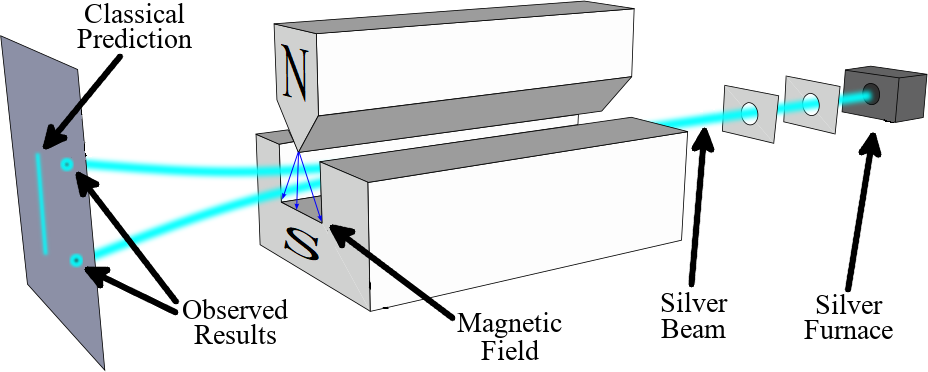
\includegraphics[width=100mm]{Stern-Gerlach_experiment_svg.png}
\caption[Caption for LOF]{The Stern-Gerlach Experiment.\protect\footnotemark}
\label{stern}
\end{figure}
\footnotetext{ Original diagram drawn by Theresa Knott. Labeling was modified for use in this dissertation. This image is licensed under the Creative Commons Attribution-Share Alike 4.0 International license. Source: https://commons.wikimedia.org/wiki/File:Stern-Gerlach\_experiment\_svg.svg}
 Now silver atoms have a property somewhat analogous to the classical notion of angular momentum. For instance, a spinning top has angular momentum as shown in figure \ref{spintop}. Angular momentum is a vector, so it has direction and magnitude. In the case of a spinning top, the direction of the angular momentum would be parallel to the axis of rotation, pointing one way or the other depending on whether the rotation was clockwise or counterclockwise. The magnitude of the angular momentum would then be proportional to the angular velocity of the spinning top. 
\begin{figure}[ht!]
\captionsetup{justification=centering}
\centering
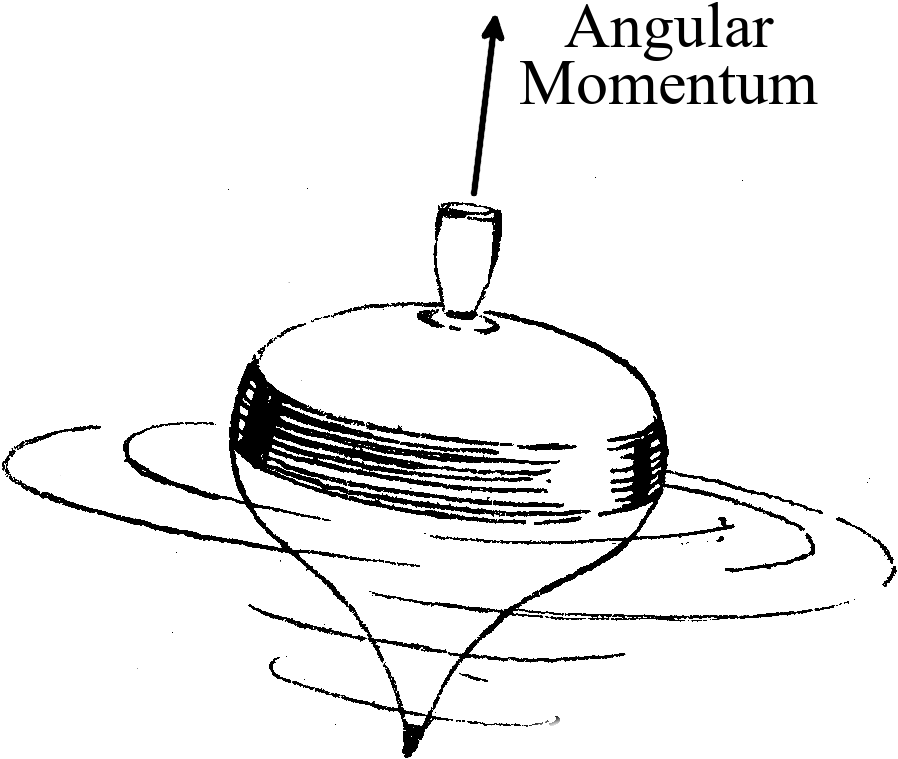
\includegraphics[width=50mm]{Top_(PSF)2.png}
\caption{Angular Momentum of a Spinning Top.\protect\footnotemark}
\label{spintop}
\end{figure}

Now if we tried to understand the angular momentum of a silver atom classically, we would expect the magnetic field of the two magnets to interact with the silver atom in a way that was determined by the relative direction of the silver atom's magnetic momentum compared to the direction of the magnetic field. Since we would expect the silver atom to have an entirely random angular momentum, we would expect it to be deflected by varying degrees either up or down in the direction of the magnetic field. Thus, if a detection screen were placed beyond the two magnets which the silver atoms would hit, we would expect there to be a whole continuum of possible locations where the silver atoms would be detected. However, in reality, it is found that there are precisely two locations where the silver atoms hit the screen. It is as though the particles can spin either clockwise or anticlockwise, but that there is absolutely no variance in the angular speed at which they rotate. This is surprising. The angular momentum appears to be \textbf{quantized} in one of two directions, either parallel to the magnetic field or antiparallel\footnotetext{Drawing by Pearson Scott Foresman, Public domain, via Wikimedia Commons. Labeling was added for use in this dissertation. Original: https://commons.wikimedia.org/wiki/File:Top\_(PSF).png.} to it.\footnote{See figure \ref{antiparallel} for what is meant be antiparallel.} Corresponding to this quantization of angular momentum, we say that the atom is either in the spin up state or the spin down state with respect to the direction of the magnetic field. 
\begin{figure}[ht!]
\captionsetup{justification=centering}
\centering
\fbox{\begin{picture}(65,50)
	\put(0,10){\vector(1,1){30}} %% a
	\put(5,25){$\vec{a}$}

	\put(65,40){\vector(-1,-1){30}} %% -a
	\put(30,25){$-\vec{a}$}
\end{picture}}
\vspace*{10px}
\caption{Meaning of antiparallel: the arrows in opposite directions are said to be antiparallel to one another.}\label{antiparallel}
\end{figure}\\
 \noindent If the direction of the magnetic field is implicitly understood, we write $\ket*{+}$ and $\ket*{-}$ for the spin up and spin down states of the atom respectively. We refer to the symbols $\ket*{+}$ and $\ket*{-}$ as \textbf{ket-vectors}, or simply as kets. We can think of the ket $\ket*{+}$ for instance as shorthand for the proposition “the particle is in the spin up state.” If we knew this proposition to be true, we would know which of the two locations on the detection screen the particle would end up if it were to travel between the two magnets of the Stern-Gerlach apparatus. If we need to specify the spin with respect to a particular direction of the magnetic field, say in the $\uvb{a}$-direction, we write the corresponding spin up and down states as $\ket*{\uvbp{a}}$ and $\ket*{\uvbm{a}}$. For convenience, we write $\uvbp{a}$ and $\uvbm{a}$ respectively for the location that the particle would hit the detection screen.  

The question then arises as to what happens when we rotate the magnetic field around the axis of the particle beam in the Stern-Gerlach experimental setup. It turns out that when we do this, the atoms are again detected in only one of two locations (see figure \ref{rotate}).
\begin{figure}[ht!]
\captionsetup{justification=justified}
\centering
\usetikzlibrary {angles, quotes, calc} 
\pgfmathsetmacro{\ang}{-20}
\begin{tikzpicture}
\tikzset{
mydot/.pic={\fill (0,0) circle (\dotsize);}}
\coordinate (a) at (0, -2.1);
\coordinate (b) at (0, 2.1);
\coordinate (o) at (0, 0);
\coordinate (c) at ($ (o)!1! \ang:(a) $);
\coordinate (d) at ($ (o)!1! \ang:(b) $);
\draw (-5, -3) rectangle (5, 3);
\draw[thick, loosely dashed]  (d) pic {mydot} node[anchor=south west]{$\uvbp{b}$} -- (o) -- (b) pic {mydot} node[anchor=south ]{$\uvbp{a}$} pic [draw=black!50!black, solid, fill=black!10, angle radius=15mm, "$\theta$"] {angle = d--o--b}; 
\draw[thick, loosely dashed] (a) pic {mydot} node[anchor=north ]{$\uvbm{a}$} -- (o) -- (c) pic {mydot} pic {mydot} node[anchor= east]{$\uvbm{b}$};
\fill (o) circle (\dotsize);

\draw[thick, solid, -stealth] (-2,0) -- (-0.2,0);
\node[text width=2cm, align=center] at (-3.2,0) {\footnotesize Beam center  of  the  silver atoms};
\node[draw] at (3,-2){Detection Screen};
\end{tikzpicture}
\vspace*{10px}
\caption{Locations of detections before and after rotating the magnetic field by an angle $\theta$. Before rotation, the particles can be detected at either location $\uvbp{a}$ or location $\uvbm{a}$. After the rotation, particles can be detected at either location $\uvbp{b}$ or $\uvbm{b}$. }
\label{rotate}
\end{figure}
\\ \noindent
So suppose we knew the particle was in a spin state such that it was on course to arrive at location $\uvbp{a}$ because we had previously directed it through another magnetic field in the $\uvb{a}$-direction. For example, see figure \ref{knownspin} for how this might be done.
\begin{figure}[ht!]
\captionsetup{justification=centering}
\centering
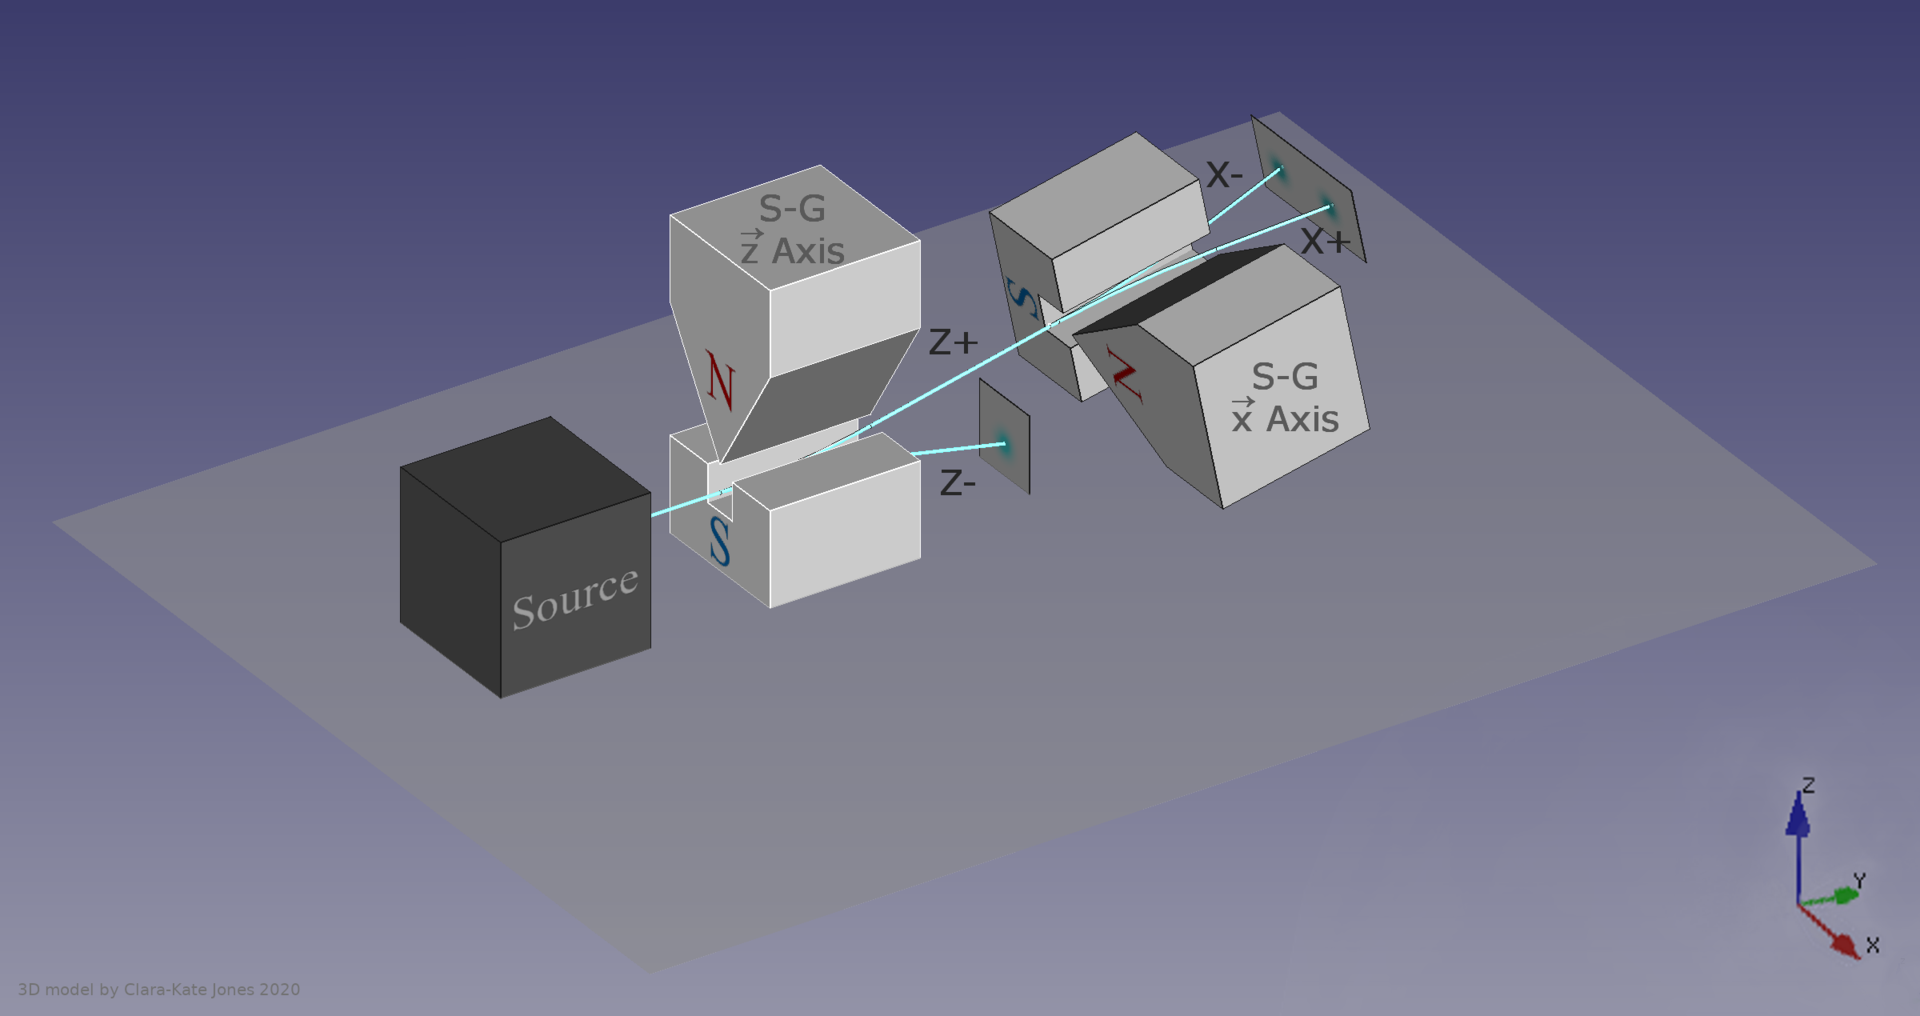
\includegraphics[width=100mm]{1920px-Stern-Gerlach_Analyzer_Sequential_Series_E2v.png}
\vspace*{10px}
\caption{Two Stern-Gerlach experiements in sequence. By directing the beam of particles through one magnetic field first, the particles emerging in one of the two beams will be in a known spin state before they enter the second magnetic field.\protect\footnotemark}
\label{knownspin}
\end{figure}
\footnotetext{Diagram by MJasK. This file is licensed under the Creative Commons Attribution-Share Alike 4.0 International license. Source: https://commons.wikimedia.org/wiki/File:Stern-Gerlach\_Analyzer\_Sequential\_Series\_E2.png. } In this experimental setup, the second magnetic field has been rotated by an angle of $90^\circ$ with respect to the first magnetic field. But suppose we just rotated the second magnetic field by a very small angle $\theta$ with respect to the first magnetic field. Then we would expect the particle now to arrive at a location  $\uvbp{b}$ close by to $\uvbp{a}$ as shown in figure \ref{rotate}. And this is what we notice experimentally for the most part. However, occasionally, the particle will arrive at location $\uvbm{b}$. The frequency of this occurrence becomes less and less the less and less the magnetic field is rotated (i.e. the smaller $\theta$ is), so that if the magnetic field is not rotated at all, i.e. $\theta=0$, the particle will always arrive at location $\uvbp{a}$. 
 To capture the probabilistic nature of these outcomes, we use the bra-ket notation. Thus, if $\ket*{\psi}$ stands for either the $\ket*{\uvbp{a}}$ or the $\ket*{\uvbm{a}}$-state, and $\ket*{\chi}$ stands for either the $\ket*{\uvbp{b}}$ or the $\ket*{\uvbp{b}}$-state, then we define the bra-ket $\ip*{\psi}{\chi}\in\mathbb{C}$ to be a complex number\footnote{With regards to the set of complex numbers $\mathbb{C}$, we will use the notation $i=\sqrt{-1}$. Complex conjugation will be denoted by an overline so that $\overline{x+iy}=x-iy$ for real numbers $x$ and $y$. The modulus of a complex number $z=x+iy$ will then be given by $\abs{z}=\sqrt{z\overline{z}}=\sqrt{x^2+y^2}.$ Since the defining property of  $\ip*{\psi}{\chi}$ is that $\abs*{\ip*{\psi}{\chi}}^2$ is the probability that the particle will be found to be in state $\ket*{\psi}$ given that we know that the particle is in state $\ket*{\chi}$, we have to choose an arbitrary phase to fully determine $\ip*{\psi}{\chi}$. } that satisfies the \textbf{Born Rule},\label{bornrule} namely $\abs*{\ip*{\psi}{\chi}}^2$ is the probability that the particle will be found to be in state $\ket*{\psi}$ given that we know that the particle is in state $\ket*{\chi}$. For example, if $\abs*{\ip*{\psi}{\chi}}^2=\frac{1}{4},$ and we performed the experiment a 1000 times with the particle initially prepared in the $\ket*{\chi}$-state, then we would expect the particle to be found in the $\ket*{\psi}$-state in around 250 runs of the experiment.   We also insist that $\ip{\psi}{\chi}=\overline{\ip{\chi}{\psi}}.$\footnote{Note that this conditions implies time symmetry: the probability a particle transitions from a state $\ket*{\chi}$ to a state $\ket*{\psi}$ will be the same as the probability a particle transitions from the state $\ket*{\psi}$ to the state $\ket*{\chi}$. This is in accord with the observation that closed quantum systems are symmetric on time-reversal. This might at first seem surprising in the light of the fact that phenomena such as radioactive decay are not obviously time-symmetric. However, it turns out that this time asymmetry results from the quantum system not being closed. For more details, see \cite{Pascazio2013}.} We would thus expect $\abs*{\ip*{\uvbp{a}}{\uvbp{a}}}^2$ to be $1$ and $\abs*{\ip*{\uvbm{a}}{\uvbp{a}}}^2$ to be $0$. It will follow that $\ip*{\uvbm{a}}{\uvbp{a}}$ has to be $0$, and that $\ip*{\uvbp{a}}{\uvbp{a}}$ has modulus $1$, but by convention we choose $\ip*{\psi}{\chi}$  such that $\ip*{\psi}{\psi}$ is a real and positive number, in which case we must have $\ip*{\uvbp{a}}{\uvbp{a}}=1$.
 If we now rotate the magnetic field by an angle $\theta$ as indicated in figure \ref{rotate}, the particle will be detected either at location $\uvbp{b}$ or location $\uvbm{b}$. We can then ask the question “given that the particle is in state $\ket*{\uvbp{a}}$, what is the probability that the particle will be found to be in state $\ket*{\uvbp{b}}$?” According to the notation discussed above, this probability will be $|\ip*{\uvbp{b}}{\uvbp{a}}|^2$ where $\ip*{\uvbp{b}}{\uvbp{a}}$ is a complex number such that $\ip*{\uvbp{b}}{\uvbp{a}}=1$ when $\theta =0$ and $\ip*{\uvbp{b}}{\uvbp{a}}=0$ when $\theta=180\degree.$ We would likewise expect $\ip*{\uvbp{b}}{\uvbm{a}}=0$ when $\theta =0$ and $\ip*{\uvbp{b}}{\uvbm{a}}=1$ when $\theta=180\degree.$ Since $\cos 0\degree = \sin 90\degree = 1$ and $\cos 90\degree = \sin 0\degree = 0$, we might guess that in general $\abs*{\ip*{\uvbp{b}}{\uvbp{a}}}=\abs*{\cos(\theta/2)}$ and  $\abs*{\ip*{\uvbp{b}}{\uvbm{a}}}=\abs*{\sin(\theta/2)}.$ Experimentation shows us that this guess is correct.
 This suggests that we can express the state $\ket*{\uvbp{b}}$ in terms of the states $\ket*{\uvbp{a}}$ and $\ket*{\uvbm{a}}$. We thus suppose that 
\begin{subequations}\label{vectoradd}
\begin{align}
\ket*{\uvbp{b}}&=\alpha\ket*{\uvbp{a}}+\beta\ket*{\uvbm{a}}\label{vectoradd1}\\
\ket*{\uvbm{b}}&=\bar{\alpha}\ket*{\uvbm{a}}-\bar{\beta}\ket*{\uvbp{a}}\label{vectoradd2}
\end{align} 
\end{subequations}
for complex numbers $\alpha, \beta \in \mathbb{C}$ such that $|\alpha|^2+|\beta|^2=1$, and we suppose that the bra-ket has the \textbf{linearity} property so that  $\ip*{\psi}{\uvbp{b}}=\alpha\ip*{\psi}{\uvbp{a}}+\beta\ip*{\psi}{\uvbm{a}}$ and $\ip*{\psi}{\uvbm{b}}=\bar{\alpha}\ip*{\psi}{\uvbm{a}}-\bar{\beta}\ip*{\psi}{\uvbp{a}}$ for any state $\ket{\psi}$. Then  it will follow that  $\ip*{\uvbp{b}}{\uvbm{b}}=0,$\footnote{To see this, by putting $\ket{\psi}=\ket*{\uvbp{b}}$, we will have $\ip*{\uvbp{b}}{\uvbm{b}}=\bar{\alpha}\ip*{\uvbp{b}}{\uvbm{a}}-\bar{\beta}\ip*{\uvbp{b}}{\uvbp{a}}$ by equation (\ref{vectoradd2}). Since  $\ip*{\uvbp{b}}{\uvbm{a}}=\overline{\ip*{\uvbm{a}}{\uvbp{b}}}$ we have $\ip*{\uvbp{b}}{\uvbm{a}}=\bar{\beta}$ by equation (\ref{vectoradd1}), and likewise, since $\ip*{\uvbp{b}}{\uvbp{a}}=\overline{\ip*{\uvbp{a}}{\uvbp{b}}}$, we have $\ip*{\uvbp{b}}{\uvbp{a}}=\bar{\alpha}.$  Therefore  $\ip*{\uvbp{b}}{\uvbm{b}}=\overline{\alpha}\overline{\beta}-\overline{\beta}{\overline{\alpha}}=0.$ }  and that $\ip*{\uvbp{b}}{\uvbp{b}}=\ip*{\uvbm{b}}{\uvbm{b}} = 1.$\footnote{To see this, by putting $\ket{\psi}=\ket*{\uvbp{b}}$ and using equation (\ref{vectoradd1}), we will have $\ip*{\uvbp{b}}{\uvbp{b}}=\alpha\ip*{\uvbp{b}}{\uvbp{a}}+\beta\ip*{\uvbp{b}}{\uvbm{a}}=\alpha\overline{\alpha}+\beta\overline{\beta}=\abs{\alpha}^2+\abs{\beta}^2=1.$ By a similar calculation, we also see $\ip*{\uvbp{b}}{\uvbp{b}}=1$.}  
If we then put  $\alpha=\cos(\theta/2)$ and $\beta=\sin(\theta/2)$, it will follow that $\abs*{\ip*{\uvbp{b}}{\uvbp{a}}}=\abs*{\cos(\theta/2)}$ and  $\abs*{\ip*{\uvbp{b}}{\uvbm{a}}}=\abs*{\sin(\theta/2)},$\footnote{To satisfy these criteria, $\alpha$ and $\beta$ are only determined up to rotation by a complex number. Rotating a complex number $z\in\mathbb{C}$ just means multiplying it by a complex number $\lambda$ of modulus $1$ (i.e. $\abs{\lambda}=1$) to get $\lambda z$. We would need to take into account this rotation factor if we considered the three-dimensional situation. Then, without loss of generality, $\alpha=\cos(\theta/2)$ and $\beta=e^{i\phi}\sin(\theta/2)$ where $\theta$ and $\phi$ are the polar and azimuthal angles respectively.} and so with these values for $\alpha$ and $\beta$ we will have
\begin{subequations}\label{spintrans}
\begin{align}
\ket*{\uvbp{b}}&= \cos(\theta/2)\ket*{\uvbp{a}}+\sin(\theta/2) \ket*{\uvbm{a}},\label{spintrans1}\\
\ket*{\uvbm{b}}&= \cos(\theta/2)\ket*{\uvbm{a}}-\sin(\theta/2) \ket*{\uvbp{a}}.\label{spintrans2}
\end{align}
\end{subequations}
\section{Hidden Variables }
Now it is tempting to suppose that the expression of $\ket*{\uvbp{b}}$ in terms of $\ket*{\uvbp{a}}$ and $\ket*{\uvbm{a}}$ merely represents our knowledge of the true spin state of a particle along the $\uvb{a}$ axis given our knowledge that it would be detected at location $\uvbp{b}$ with probability $1$ should we decide to measure the particle's state along the $\uvb{b}$-axis. If we were to make this supposition, there would be a fact of the matter, albeit unknown to us, concerning what spin state the particle would be found to be in  were we to measure its spin along the $\uvb{a}$-axis. And  even though we might decide not to measure the spin of the particle along the $\uvb{a}$-axis, there would still be this hidden fact about the particle's spin in this direction. And given this supposition, since there would be no reason to suppose there was anything special about the $\uvb{a}$-axis, it would then be reasonable to suppose that there were hidden facts about what spin direction the particle would be found to be in for every possible axis orientation. This would mean that a complete description of the particle's spin state would require an infinite list of outcomes for all the possible orientations we could configure the magnetic field of our Stern-Gerlach apparatus. Given this assumption, as well as the assumption that it is already known that the particle would be detected at $\uvbp{b}$, a complete description of the particle's  state could be depicted as $\ket*{\uvbp{a},\uvbp{b},\ldots}$ or  $\ket*{\uvbm{a},\uvbp{b},\ldots}$, etc. where the ellipses would range over one of the two possible measurement outcomes for every other magnetic field orientation. However, because we would never in practice be able to perform all these experiments, and since only one such experiment would be needed to alter this infinite list,\footnote{In other words, it is assumed that directly measuring the particle will involve perturbing it so that its state will change.} nearly all of the entries in this infinite list would remain forever hidden. Hence, this would be an example of a \textbf{hidden variables} interpretation of quantum theory.  
\section{Bell's Inequality}\label{BellSection}
Now although a hidden variables interpretation seems rather intuitive, a problem arises when two spin particles are coupled together with each other. This problem is known as the \textbf{EPR paradox.}\footnote{For more details of this problem, see \cite[241-249]{Sakurai}.} To explain how this problem arises, we need to consider two identical fermionic particles that are coupled together. Fermions have the property that no two particles that are coupled together can be in exactly the same spin state. Thus, if we call our fermionic particles $q_A$ and $q_B$, and suppose particle $q_A$ was in the state $\ket*{\uvbp{a},\uvbp{b},\uvbm{c},\ldots}$, then on the assumption that making a measurement on particle $q_A$ has no effect on the state of particle $q_B$, it would follow that particle $q_B$ would be in the  state  $\ket*{\uvbm{a},\uvbm{b},\uvbp{c},\ldots}$. It is thus appropriate to refer to the spin directions describing $q_A$ and $q_B$ as \textbf{local hidden variables}. It seems very natural to assume these  hidden variables are local. This assumption is a special case of \textbf{Einstein's locality principle}: For two spatially separated systems $S_1$ and $S_2$,  the real factual situation of the system $S_2$ should be independent of what is done to the system $S_1$.\footnote{Einstein expressed this locality principle in his autobiographical notes: ``But on one supposition we should, in my opinion, absolutely hold fast: the real factual situation of the system $S_2$ is independent of what is done with the system $S_1$, which is spatially separated from the former.''\cite[p. 85]{EinsteinLocality}.} 
 
We now suppose we have an experimental setup so that in each run of the experiment, we have two fermionic particles $q_A$ and $q_B$,  and particle $q_A$ is sent to Alice who measures $q_A$'s spin in a direction of her choosing, and particle $q_B$ is sent to Bob who measures $q_B$'s spin in a direction of his choosing. We assume that in each run of the experiment, Alice and Bob independently measure the spin of their particles along one of three possible directions $\uvb{a}$, $\uvb{b}$, and $\uvb{c}$, and that Einstein's locality principle holds. Furthermore, we assume that in each run of the experiment, the outcome of Alice's measurement will be statistically independent of any of the other measurement outcomes for different runs of the experiment, and for any of the three axes she measures along, she will get a spin up outcome or a spin down outcome with equal probability of $\frac{1}{2}.$ Likewise, we assume Bob's measurement outcomes are also similarly independent between different runs of the experiment. We also assume that the $8=2^3$ states $\ket*{\uvbpm{a},\uvbpm{b},\uvbpm{c}}_A$ exhaust all the possible states for Alice's particles that can be distinguished from one another by one of the three possible measurements she can make. Thus, Alice can distinguish between the $\ket*{\uvbp{a},\uvbp{b},\uvbp{c}}_A$-state and the $\ket*{\uvbp{a},\uvbp{b},\uvbm{c}}_A$-state by making a measurement along the $\uvb{c}$-axis, though if she happened to make her measurement along the $\uvb{a}$ or $\uvb{b}$-axis, she wouldn't be able to distinguish between these two states. But in principle, she can distinguish between these two states if she happens to make her measurement along the right axis, in this case the $\uvb{c}$-axis. We similarly assume the states $\ket*{\uvbpm{a},\uvbpm{b},\uvbpm{c}}_B$  exhaust all the possible states for Bob's particles that he can distinguish between, and we assume that if Alice and Bob measure the particle along the same axis, they will always obtain opposite results from one another. For instance, if Alice's particle is in state $\ket*{\uvbp{a},\uvbp{b},\uvbp{c}}_A$, then Bob's particle must be in state $\ket*{\uvbm{a},\uvbm{b},\uvbm{c}}_B$. Now suppose the experiment is run $N$ times for large $N$,\footnote{$N$ has to be large since a frequentist definition of probability is being assumed.} and let $N_i$ be the number of times particle $q_A$ is in the $i$th state so that\footnote{The notation $\sum_{i=1}^8 N_i$ is shorthand for $N_1+N_2+N_3+N_4+N_5+N_6+N_7+N_8$.} $N=\sum_{i=1}^8 N_i$ as shown in table \ref{hiddentable}.

\begin{table}[ht]
\caption{Spin-components of particles $q_A$ and $q_B$ in the hidden variable theory}
\centering
\begin{tabular}{c c c} 
\\ 
\hline
\textbf{Population}& \textbf{Particle} $\bm{q_A}$ & \textbf{Particle} $\bm{q_B}$ \\ [0.5ex] 
\hline
$N_1$ & $\ket*{\uvbp{a},\uvbp{b},\uvbp{c}}_A$ & $\ket*{\uvbm{a},\uvbm{b},\uvbm{c}}_B$ \\ 

$N_2$ & $\ket*{\uvbp{a},\uvbp{b},\uvbm{c}}_A$ & $\ket*{\uvbm{a},\uvbm{b},\uvbp{c}}_B $\\ 

$N_3$ & $\ket*{\uvbp{a},\uvbm{b},\uvbp{c}}_A$ & $\ket*{\uvbm{a},\uvbp{b},\uvbm{c}}_B$ \\ 

$N_4$ & $\ket*{\uvbp{a},\uvbm{b},\uvbm{c}}_A$ & $\ket*{\uvbm{a},\uvbp{b},\uvbp{c}}_B $\\ 

$N_5$ & $\ket*{\uvbm{a},\uvbp{b},\uvbp{c}}_A$ & $\ket*{\uvbp{a},\uvbm{b},\uvbm{c}}_B$ \\ 

$N_6$ & $\ket*{\uvbm{a},\uvbp{b},\uvbm{c}}_A$ & $\ket*{\uvbp{a},\uvbm{b},\uvbp{c}}_B$ \\ 

$N_7$ & $\ket*{\uvbm{a},\uvbm{b},\uvbp{c}}_A$ & $\ket*{\uvbp{a},\uvbp{b},\uvbm{c} }_B$\\ 

$N_8$ & $\ket*{\uvbm{a},\uvbm{b},\uvbm{c}}_A$ & $\ket*{\uvbp{a},\uvbp{b},\uvbp{c}}_B$ \\ 
\hline
\end{tabular}
\label{hiddentable}
\end{table}
 We define $P_{AB}(\uvbp{a};\uvbp{b})$ to be the probability that Alice measures particle $q_A$ to be at location $\uvbp{a}$ on her detection screen and Bob measures particle $q_B$ to be at location $\uvbp{b}$ on his detection screen. We similarly define the probabilities for all other combinations of detection locations. It is relatively easy to calculate all these probabilities in terms of the values $N_i$ from table \ref{hiddentable},\footnote{e.g.  $P_{AB}(\uvbp{a};\uvbp{b})=\frac{N_3+N_4}{N},\, P_{AB}(\uvbp{a};\uvbp{c})=\frac{N_2+N_4}{N},\,P_{AB}(\uvbp{c};\uvbp{b})=\frac{N_3+N_7}{N}$  } or alternatively by simply measuring the frequency of these different outcomes for where Alice and Bob detect their particles. Although the values of $N_i$ are unknown, on the assumption that there is a fact of the matter of which states in table \ref{hiddentable} obtain, and on the assumption that the states to which the $N_i$ correspond exhaust all the possible states for Alice's and Bob's particles, we can show that\footnote{This inequality follows since $P_{AB}(\uvbp{a};\uvbp{b})=\frac{N_3+N_4}{N}\leq \frac{N_2+N_4+N_3+N_7}{N}=P_{AB}(\uvbp{a};\uvbp{c})+P_{AB}(\uvbp{c};\uvbp{b})$.}
 \begin{equation}\label{bellinequality}
P_{AB}(\uvbp{a};\uvbp{b})\leq P_{AB}(\uvbp{a};\uvbp{c})+P_{AB}(\uvbp{c};\uvbp{b}).
\end{equation}
This inequality is known as \textbf{Bell's inequality}, and it follows from Einstein's locality principle.  However, it turns out that when this experiment is actually performed, Bell's inequality is violated. Because of this violation, the most natural conclusion to draw is that it is wrong to suppose that there any hidden variables describing possible spin measurement outcomes. But it also turns out that this violation of Bell's inequality is entirely predictable if we assume that when the two particles $q_A$ and $q_B$ are coupled together, everything that can be said about their spins is encoded in the so called \textbf{Bell state}: 
\begin{equation}\label{bell}
\frac{1}{\sqrt{2}}(\ket*{\uvbp{a}}_A\ket*{\uvbm{a}}_B-\ket*{\uvbm{a}}_A\ket*{\uvbp{a}}_B).\end{equation}
This state means that if both Alice and Bob measure their particles along the measurement axis $\uvb{a}$, then with probability $\frac{1}{2}$, Alice will detect her particle at location $\uvbp{a}$ and Bob will detect his particle at location $\uvbm{a}$. Likewise, with probability $\frac{1}{2}$, Alice will detect her particle at location $\uvbm{a}$ and Bob will detect his particle at location $\uvbp{a}$. Prima facie, it looks like the Bell state depends on the direction of $\uvb{a}$. However it can be shown that for any other direction $\uvb{b}$,
\begin{equation}\label{bellstate2}\frac{1}{\sqrt{2}}(\ket*{\uvbp{a}}_A\ket*{\uvbm{a}}_B-\ket*{\uvbm{a}}_A\ket*{\uvbp{a}}_B)=\frac{1}{\sqrt{2}}(\ket*{\uvbp{b}}_A\ket*{\uvbm{b}}_B-\ket*{\uvbm{b}}_A\ket*{\uvbp{b}}_B).\protect\footnotemark\end{equation}
\footnotetext{To see this, using the transformation rules given in equation (\ref{spintrans}) we have 
\begin{align*}\frac{1}{\sqrt{2}}(\ket*{\uvbp{b}}\ket*{\uvbm{b}}-\ket*{\uvbm{b}}\ket*{\uvbp{b}})&=\frac{1}{\sqrt{2}}((\cos(\theta/2)\ket*{\uvbp{a}}+\sin(\theta/2)\ket*{\uvbm{a}})(\cos(\theta/2)\ket*{\uvbm{a}}-\sin(\theta/2)\ket*{\uvbp{a}})\\
&\quad-(\cos(\theta/2)\ket*{\uvbm{a}}-\sin(\theta/2)\ket*{\uvbp{a}})(\cos(\theta/2)\ket*{\uvbp{a}}+\sin(\theta/2)\ket*{\uvbm{a}}))\\ 
&=\frac{1}{\sqrt{2}}(\cos(\theta/2)\ket*{\uvbp{a}}\cos(\theta/2)\ket*{\uvbm{a}}-\cos(\theta/2)\ket*{\uvbp{a}}\sin(\theta/2)\ket*{\uvbp{a}}\\
&\quad+\sin(\theta/2)\ket*{\uvbm{a}}\cos(\theta/2)\ket*{\uvbm{a}}-\sin(\theta/2)\ket*{\uvbm{a}}\sin(\theta/2)\ket*{\uvbp{a}}\\
&\quad-\cos(\theta/2)\ket*{\uvbm{a}}\cos(\theta/2)\ket*{\uvbp{a}}-\cos(\theta/2)\ket*{\uvbm{a}}\sin(\theta/2)\ket*{\uvbm{a}}\\
&\quad+\sin(\theta/2)\ket*{\uvbp{a}}\cos(\theta/2)\ket*{\uvbp{a}}+
\sin(\theta/2)\ket*{\uvbp{a}}\sin(\theta/2)\ket*{\uvbm{a}})\\
&=\frac{1}{\sqrt{2}}((\cos[2](\theta/2)+\sin[2](\theta/2))\ket*{\uvbp{a}}\ket*{\uvbm{a}}\\
&\quad-(\cos[2](\theta/2)+\sin[2](\theta/2))\ket*{\uvbm{a}}\ket*{\uvbp{a}})\\
&=\frac{1}{\sqrt{2}}(\ket*{\uvbp{a}}\ket*{\uvbm{a}}-\ket*{\uvbm{a}}\ket*{\uvbp{a}}).
\end{align*}}Thus, without loss of generality we can write the joint state of both Alice and Bob's particles as in equation (\ref{bell}), from which it would follow that 
\begin{equation*}
P_{AB}(\uvbp{a};\uvbp{b})=\frac{1}{2}\sin^2(\theta/2)
\end{equation*}
where $\theta$ is the angle between the $\uvb{a}$-axis and $\uvb{b}$-axis.\footnote{To see why this is, let $P_A(\uvbp{a})$ be the probability that Alice would detect her particle at location $\uvbp{a}$ given that she is making a measurement along the $\uvb{a}$-axis, and let $P_{BA}(\uvbp{b}|\uvbp{a})$ be the probability that Bob will detect his particle at location $\uvbp{b}$ given that he is making a measurement along the $\uvb{b}$-axis and Alice has detected her particle at location $\uvbp{a}$. Given that the joint state of the particles is given by equation (\ref{bell}), $P_A(\uvbp{a})=\frac{1}{2}.$ But also note that if  Alice has detected her particle at location  
$\uvbp{a}$, then Bob's particle must be in state $\ket*{\uvbm{a}}$. From the Born Rule (see page \pageref{bornrule}) and equation (\ref{spintrans1}) it follows that 
$$P_{BA}(\uvbp{b}|\uvbp{a})= |\ip*{\uvbp{b}}{\uvbm{a}}|^2=\sin^2(\theta/2).$$ 
Therefore, $$P_{AB}(\uvbp{a};\uvbp{b})= P_A(\uvbp{a})P_{BA}(\uvbp{b}|\uvbp{a})=\frac{1}{2}\sin^2(\theta/2).$$} Then taking the angle between the $\uvb{a}$ and $\uvb{b}$-axes to be $90^\circ$, and the $\uvb{c}$-axis to be at $45^\circ$ to both the $\uvb{a}$ and $\uvb{b}$-axes, we would find that $P_{AB}(\uvbp{a};\uvbp{b})=\frac{1}{4}$ and $P_{AB}(\uvbp{a};\uvbp{c})+P_{AB}(\uvbp{c};\uvbp{b})=0.1464\ldots$, and so Bell's inequality would be violated if we assumed that the probability of each outcome is determined by the Bell state  (\ref{bell}). 
\section{The Copenhagen Interpretation}
 The experiment described in the previous section implies that the behavior of Alice's and Bob's particles can't be explained in terms of local hidden variables. But this experiment also calls into question the Copenhagen interpretation of quantum physics. To explain the Copenhagen interpretation and what is problematic about it, suppose Alice has a measurement device which we will denote by $\Lambda_{\uvbp{a}}$\label{Lambdaa} and which outputs the number 1 when her particle is detected at location $\uvbp{a}$, and outputs 0 when her particle is detected at location $\uvbm{a}$. Given that Alice knows that the state of both particles together is given by equation (\ref{bell}), she can work out the expectation value of her measurement $\ev*{\Lambda_{\uvbp{a}}}$ by summing up the product of each probability measurement outcome with the value of each measurement. This will give an expectation value of $\ev*{\Lambda_{\uvbp{a}}}=\frac{1}{2}\times 1 + \frac{1}{2}\times 0 = \frac{1}{2}.$ More generally, if Alice had a measuring device $\Lambda$ with $N$ measurement outcome values $\lambda_1,\ldots,\lambda_N$ and with respective probabilities $p_1,\ldots,p_N$ so that $\sum_{i=1}^N p_i=1,$ then the expectation $\ev*{\Lambda}$ would be given by the formula
\begin{equation}\label{expectation}\ev*{\Lambda} =\sum_{i=1}^N p_i\lambda_i.
\end{equation}
Now given that there are no hidden variables and that equation (\ref{bell}) encodes everything that can be said about the spins of the two particle system, it is tempting to suppose that the expectation value $\ev*{\Lambda_{\uvbp{a}}}$ tells us something objective about the system rather than just something about Alice's state of knowledge about the system.  Given this assumption, there then arises the question of what happens when a measurement is made. According to the Copenhagen interpretation, when Bob makes his measurement, the quantum state collapses to a component of the quantum state corresponding to the measurement Bob makes. Thus, if Bob's measurement device $\Lambda_{\uvbm{a}}$ outputs the number $1$, (i.e. Bob's particle is detected at location $\uvbm{a}$), then the state of the combined system would change accordingly as:
$$\frac{1}{\sqrt{2}}(\ket*{\uvbp{a}}_A\ket*{\uvbm{a}}_B-\ket*{\uvbm{a}}_A\ket*{\uvbp{a}}_B)\xrightarrow{\text{Collapse!!}}\ket*{\uvbp{a}}_A\ket*{\uvbm{a}}_B $$
If Bob makes his measurement first with his measurement device $\Lambda_{\uvbm{a}}$  outputting $1$, then with probability $1$ Alice's measurement device $\Lambda_{\uvbp{a}}$ will output $1$. Hence, once Bob has made this measurement, then the expectation value for Alice's measurement will be $\ev*{\Lambda_{\uvbp{a}}}=1.$ Thus, the expectation value for Alice's measurement device changes from $\frac{1}{2}$ to $1$ when Bob makes his measurement.
 
Now the problem\label{Copenhagenproblem} with this change in expectation value for Alice's measurement is that it will depend on whether Bob performs his measurement first or whether Alice performs her measurement first. But according to Einstein's theory of relativity, who performs their measurement first will depend on which inertial frame of reference one is in.\footnote{In Special Relativity, an inertial frame of reference is a space-time coordinate system $(t, x, y, z)$ in which all objects which have no forces acting on them have trajectories that are straight lines. Thus, we can move to another inertial frame by moving to a reference frame with constant velocity $\vb{v}$ with respect to the first reference frame. In the case when $\vb{v}=(v, 0, 0)$, Einstein's theory of Special Relativity tells us that under such a “boost”, space-time coordinates will transform as $(t,\vb{x})\rightarrow(t',x',y',z')=(\gamma\big(t - \frac{vx}{c^2}\big),\gamma(x-vt),y,z)$ where $c$ is the speed of light and $\gamma=\Big(\sqrt{1-\frac{v^2}{c^2}}\Big)^{-1}.$ } Thus, if we are moving at one velocity, it may appear that Alice makes her measurement first, whereas if we are moving at another velocity, it may appear that Bob makes his measurement first. This suggests the expectation values for Alice and Bob's measuring devices will depend on which frame of reference we are in. However, Einstein's theory of relativity tells us that scalar quantities such as the expectation values for Alice and Bob's measuring devices should be independent of which inertial frame we are in. 

Now many physicists would be loath to reject Einstein's theory of relativity. At the same time, many physicists are also convinced by the violation of Bell's inequality that there are no hidden variables for the spin states of particles, and hence they are convinced that the Bell state is not just a description of someone's epistemic state: rather it is a complete physical description of two coupled fermionic particles with regard to their spins. The way many physicists seek to resolve this tension between Einstein's theory of relativity and the violation of Bell's inequality is to deny the Copenhagen interpretation of quantum physics so that there is no quantum state collapse. But if one denies that there is any quantum state collapse and denies that there are any hidden variables, the question then arises of how is one  meant to interpret the quantum state? 
 \section{A preliminary consideration of the many-worlds interpretation}
 At this stage in the line of reasoning, it is too early to resort to a many-worlds interpretation of the Bell state where  the first component corresponds to a world in which Alice detects her particle at location $\uvbp{a}$ and Bob detects his particle at location $\uvbm{a}$, and where the second component corresponds to a world in which Alice detects her particle at location $\uvbm{a}$ and Bob detects his particle at location $\uvbp{a}$. The reason such an interpretation would be premature  is  because as mentioned on page \pageref{bellstate2}, for any other axis $\uvb{b}$, the transformation rules in equation (\ref{spintrans}) imply that
\begin{equation*}\frac{1}{\sqrt{2}}(\ket*{\uvbp{a}}_A\ket*{\uvbm{a}}_B-\ket*{\uvbm{a}}_A\ket*{\uvbp{a}}_B)=\frac{1}{\sqrt{2}}(\ket*{\uvbp{b}}_A\ket*{\uvbm{b}}_B-\ket*{\uvbm{b}}_A\ket*{\uvbp{b}}_B).\end{equation*}
Similarly, given the transformation rules in equation (\ref{spintrans}), we should resist the temptation  to interpret a state of the form $\frac{1}{\sqrt{2}}(\ket*{\uvbp{a}}+\ket*{\uvbm{a}})$ as representing two worlds, one in which the particle is in the state $\ket*{\uvbp{a}},$ and another in which the particle is in the state $\ket*{\uvbm{a}}.$ For according to equation (\ref{spintrans1}), the much more obvious interpretation is that this state just describes one world in which the particle is in the state $\ket*{\uvbp{b}}$ where the angle between
 the $\uvb{a}$ and the  $\uvb{b}$ axis is $90\degree$.\footnotemark
 
In order to make a case for a many-worlds interpretation, we need to discuss decoherence theory. Decoherence theory considers how a system interacts with its environment, and it allows us to understand what kinds of measurements can be made on the system. In order to discuss decoherence theory and its relevance to the many-worlds interpretation, we first need to introduce the mathematical formalism of quantum mechanics.

\section{The mathematical formalism of quantum mechanics}
 Given\footnotetext{This is because when $\theta=90\degree$, $\sin(\theta/2)=\cos(\theta/2)=\frac{1}{\sqrt{2}}$, so  $\ket*{\uvbp{b}}= \frac{1}{\sqrt{2}}(\ket*{\uvbp{a}}+\ket*{\uvbm{a}})$ in equation (\ref{spintrans1}) with $\theta=90\degree$. } a possible kind of measurement (e.g. measuring the spin of a particle along a particular axis), there will be a mathematical object called an \textbf{observable} which encodes all the possible measurement outcomes for this particular kind of measurement. The precise mathematical definition of an observable is as follows: an observable of a physical system is a Hermitian operator that acts on the Hilbert space of states describing the physical system. In order to understand what this definition means, there are a number of things we need to explain: what a Hilbert space is, what a Hermitian operator is, and how a Hermitian operator relates to a particular kind of measurement. In order to explain all this, it will be helpful to keep in mind the simple example of the measurement device $\Lambda_{\uvbp{a}}$ described on page \pageref{Lambdaa} which returns 1 if a particle is in the spin $\ket{\uvbp{a}}$-state and 0 if the particle is in the spin $\ket{\uvbm{a}}$-state. This measurement will have a corresponding observable which we will denote by $\hat{\Lambda}_{\uvbp{a}}$. 

Now we have seen that states $\ket*{\uvbp{a}}$ and $\ket*{\uvbm{a}}$ representing the spin of  a particle can be added to give the spin state $\ket*{\uvbp{b}}$ and $\ket*{\uvbm{b}}$ as seen in equation (\ref{spintrans}). We have also seen that if we have two states $\ket{\psi}$ and $\ket{\chi}$, we can define their bra-ket $\ip*{\chi}{\psi}$ to be a complex number satisfying the Born Rule so that $\abs{\ip*{\chi}{\psi}}^2$ is the probability $P(\chi|\psi)$ that the particle will be found to be in state $\ket*{\chi}$ given that we know that the particle is in state $\ket*{\psi}$. We thus imposed the assumption that  $\ip*{\psi}{\psi}=1$ for any state $\ket*{\psi}$. 

Now in order to arrive at a definition of a Hilbert space, we first need to relax this normalization condition $\ip*{\psi}{\psi}=1$. Thus, if $\ket{\psi}$  is a state and $\lambda\in\mathbb{C}$ is any non-zero complex number, then we allow $\ket{\psi'}=\lambda\ket{\psi}$ also to be a state with the caveat that $\ket{\psi'}$ represents exactly the same physical state as $\ket{\psi}$, and that $\ip*{\psi'}{\psi'}=|\lambda|^2\ip*{\psi}{\psi}.$ We define $\norm{\psi}=\sqrt{\ip*{\psi}{\psi}}$ and we say that $\ket{\psi}$ has been \textbf{normalized} when $\norm{\psi}=1$. Now when calculating probabilities, we need to remember to include a normalization factor. Thus, the probability that the particle will be found to be in state $\ket*{\chi}$ given that we know that the particle is in state $\ket*{\psi}$ will now be $P(\chi|\psi) = \frac{|\ip*{\chi}{\psi}|^2}{\norm{\psi}\norm{\chi}}.$\footnote{ If there is no such normalization factor because $\norm{\psi}=0,$ then $\ket*{\psi}$ does not represent a physical state, so the probability the system is ever in this state will be zero, and so in this case we will set $P(\chi|\psi)=0.$} It is  dropping the assumption $\norm{\psi}=1$ on the states of a physical system that gives rise to the mathematical structure known as a Hilbert Space.   

A \textbf{Hilbert space} is a set $H$ in which 
\begin{enumerate}[noitemsep, nosep, topsep=0pt]
\item any two members of $H$ can be added to obtain another member of $H$, 
\item any member of $H$ can be multiplied by any complex number to obtain another member of $H$,
\item one can take the bra-ket of any two members of $H$ to obtain a complex number\end{enumerate}
subject to some natural axioms.\footnotemark

A very simple example of a Hilbert space would be the set of states 
$$\{\alpha\ket*{\uvbp{a}}+\beta\ket*{\uvbm{a}}:\alpha,\beta\in\mathbb{C}\}.$$ 
As we will soon see, the observable corresponding to the measurement device $\Lambda_{\uvbp{a}}$ will be the operator $\hat{\Lambda}_{\uvbp{a}}$ that sends the state $\alpha\ket*{\uvbp{a}}+\beta\ket*{\uvbm{a}}$ to the state $\alpha\ket*{\uvbp{a}}.$

More generally, suppose we have an experimental setup (for example the Stern-Gerlach experiment) where a physical system can be in one of several measurable states $\ket{\psi_1},\ldots,\ket{\psi_N}\in H$. The physical system could also be in a state described by a sum of some of the $\ket{\psi_1},\ldots,\ket{\psi_N}$, \footnotetext{More formally, a complex Hilbert space $H$ is a complex vector space possessing a bra-ket. By a \textbf{complex vector space}, we mean a set $V$ such that the following axioms are satisfied 
\begin{itemize}[topsep=0pt]
\item $\psi+(\chi+\zeta)=(\psi+\chi)+\zeta,\,\forall \lambda, \chi,\zeta\in V$
\item $\psi+\chi=\chi+\psi,\,\forall \psi,\chi\in V$
\item there exists an element $\bm{0}\in V$ such that $\psi+\bm{0}=\psi,\,\forall\psi\in V$.
\item $\forall \psi\in V$ there exists an element $-\psi\in V$ such that $\psi+(-\psi)=\bm{0}$.
\item $\forall \lambda,\mu\in\mathbb{C}$ (i.e. in the set of complex numbers -- this is why it is called a \emph{complex} vector space), and $\psi\in V,\,\lambda(\mu\psi)=(\lambda\mu)\psi$.
\item for the scalar $1\in\mathbb{C},\, 1\psi=\psi,\,\forall\psi\in V$
\item $\lambda(\psi+\chi)=\lambda\psi+\lambda\chi,\forall\psi,\chi\in V$ and $\lambda\in\mathbb{C}$
\item $(\lambda+\mu)\psi=\lambda\psi+\mu\psi,\,\forall \lambda,\mu\in \mathbb{C}$ and $\psi\in V.$
\end{itemize}
A \textbf{Hilbert space} $H$ is a complex vector space possessing a bra-ket. Strictly speaking, a Hilbert space also has a property called completeness, but this property need not concern us here. In quantum theory, elements of $H$ are expressed in terms of kets, $\ket{\cdot}$. Kets behave like vectors, so for $\ket{\psi},\ket{\chi}\in H$ and $\lambda,\mu\in\mathbb{C}$, we have $\lambda\ket{\psi}+\mu\ket{\chi}=\ket{\lambda\psi+\mu\chi}$. The bra-ket of $\ket{\psi}$ and $\ket{\chi}$ is then written as $\ip{\psi}{\chi}$, and it satisfies the following axioms:
\begin{itemize}[topsep=0pt]
\item $\ip{\psi}{\chi}\in\mathbb{C},\,\forall\psi,\chi\in H$.
\item $\ip{\psi}{\chi}=\overline{\ip{\chi}{\psi}},\,\forall\psi,\chi\in H$.
\item $\ip{\psi}{\psi}\geq 0,\, \forall \ket{\psi}\in H$ and $\ip{\psi}{\psi}=0$ if and only if $\ket{\psi}=\bm{0}$.
\item $\ip{\zeta}{\lambda\psi+\mu\chi}=\lambda\ip{\zeta}{\psi}+\mu\ip{\zeta}{\chi},\,\forall \ket{\psi},\ket{\chi},\ket{\zeta}\in H$ and  $\lambda,\mu\in\mathbb{C}$.
\end{itemize}} but by saying the system is in one of these $\ket{\psi_1},\ldots,\ket{\psi_N}$ measurable states, we mean that there is a measuring device that will always give the same measurement outcome whenever the system is in the same measurable state.\footnote{When the state is described as a non-trivial sum of the measurable states, we no longer have such certainty, and instead we can only speak of probabilities based on the coefficients on the measurable states.} We also assume \textbf{orthonormality}, that is we assume $\ip{\psi_i}{\psi_i}=1$ and $\ip{\psi_i}{\psi_j}=0$ for $i\neq j$ so that if the system is measured to be in the $\ket{\psi_j}$-state, then there would be zero probability that it could then be measured to be in the $\ket{\psi_i}$-state for $i\neq j$.  

Now suppose that for each measurable state $\ket{\psi_i}$, we assign a real number $\lambda_i$.  There might be a very natural way of doing this, such as assigning  $\lambda_i$ to be the angle by which a pointer of a measurement device is deflected when the system is in the state $\ket{\psi_i}$, but the assignment could be as ad hoc as we wished – we can just think of it as the measurement value an experimenter records when he or she observes a particular measurement outcome. Given such an assignment of measurement values, the corresponding observable $\hat{\Lambda}$ would be a mapping of states to states satisfying the following rules:
\begin{enumerate}[noitemsep, nosep, topsep=0pt]
\item $\hat{\Lambda}\ket{\psi_i}=\lambda_i\ket{\psi_i}$
\item $\hat{\Lambda}(\lambda\ket{\psi}+\mu\ket{\chi})=\lambda\hat{\Lambda}\ket{\psi}+\mu\hat{\Lambda}\ket{\chi}$  for all states $\ket{\psi},\ket{\chi}\in H$ and complex numbers $\lambda,\mu\in\mathbb{C}$.
\end{enumerate}
When a mapping $\hat{\Lambda}$ satisfies rule 2., we refer to $\hat{\Lambda}$ as an \textbf{operator} on $H$. Since the measurement device $\Lambda_{\uvbp{a}}$ outputs a value of $1$ when the particle is in the $\ket*{\uvbp{a}}$-state and $0$ when the particle is in the $\ket*{\uvbm{a}}$-state, it is now clear from rule 1 and 2 why the corresponding observable $\hat{\Lambda}_{\uvbp{a}}$ will be the operator that sends the state $\alpha\ket*{\uvbp{a}}+\beta\ket*{\uvbm{a}}$ to $\alpha\ket*{\uvbp{a}}$.

For a given physical state $\ket{\psi}\in H$, we define the expected measurement value of $\hat{\Lambda}$
\begin{equation}\label{expectation2}
\ev*{\hat{\Lambda}}_\psi\myeq\sum_{i=1}^N p_i\lambda_i,
\end{equation}
just as in the formula (\ref{expectation}). Clearly, this expectation value will depend on the state the system is in, hence the subscript $\psi$. For instance, if the system is in the $\ket{\psi_i}$-state, then the expectation value of the measurement will be $\lambda_i$ since the probability that the state is in the state $\ket{\psi_i}$ will be 1, so that $p_i=1$ and $p_j=0$ for all $j\neq i$. But if the system was in an arbitrary state $\ket{\psi}=\sum_{i=1}^N \alpha_i\ket{\psi_i}$ with $\norm{\psi}=1$, then it turns out that 
\begin{equation}\refstepcounter{equation}\label{evev}\ev*{\hat{\Lambda}}_\psi=\ev*{\hat{\Lambda}}{\psi}.\tag{\theequation}\protect\footnotemark
\end{equation}\footnotetext{\label{footnote_1}To see this, note that $\alpha_i=\ip{\psi_i}{\psi}$ from which it follows that  if we define the mapping $I=\sum_{i=1}^N\dyad{\psi_i}$ then $I\ket{\psi}=\sum_{i=1}^N\ket{\psi_i}\ip{\psi_i}{\psi}=\sum_{i=1}^N\ip{\psi_i}{\psi}\ket{\psi_i}=\ket{\psi}$. Therefore,
\begin{align*}\ev*{\hat{\Lambda}}{\psi}&= \ev*{\hat{\Lambda} I}{\psi}=\sum_{i=1}^N \mel{\psi}{\hat{\Lambda}}{\psi_i}\ip{\psi_i}{\psi}=\sum_{i=1}^N\lambda_i\ip{\psi}{\psi_i}\ip{\psi_i}{\psi}\\&=\sum_{i=1}^N\lambda_i\abs{\ip{\psi_i}{\psi}}^2=\sum_{i=1}^N\lambda_ip_i=\ev*{\hat{\Lambda}}_\psi.\end{align*}}We can see that this formula is correct in the simple example when the system is in the $\ket{\psi_i}$-state, for in this case, the expectation value should be $\lambda_i$, and we clearly have $\ev*{\hat{\Lambda}}{\psi_i}=\lambda_i$ since $\hat{\Lambda}\ket{\psi_i}=\lambda_i\ket{\psi_i}$ and $\ip*{\psi_i}=1$. Hence, $\ev*{\hat{\Lambda}}_{\psi_i}=\ev*{\hat{\Lambda}}{\psi_i}$ as expected.

To say that $\hat{\Lambda}$ is \textbf{Hermitian} is to say that $\ev*{\hat{\Lambda}}{\psi}$ is a real number for any arbitrary state $\ket*{\psi}$. Thus, the observable $\hat{\Lambda}$ defined by the two criteria above is a Hermitian operator acting on the Hilbert space of states $H$. Roughly speaking, we can assume\footnote{Strictly speaking, we require a Hermitian operator to have a property known as compactness for this assumption to hold.}  that given a Hermitian operator $\hat{\Lambda}$ on a Hilbert space of states $H$, any state $\ket{\psi}\in H$ can be expressed as a (possibly infinite) sum 
\begin{equation}\label{span}
\ket{\psi}=\sum_{i=1}^N\alpha_i\ket{\psi_i}
\end{equation}
 where $\hat{\Lambda}\ket{\psi_i}=\lambda_i\ket{\psi_i}$ for some set of states $\ket{\psi_i}$ referred to as \textbf{eigenstates} of $\hat{\Lambda}$, and real numbers $\lambda_i$ referred to as \textbf{eigenvalues} of $\hat{\Lambda}$ . We will typically assume that the $\ket{\psi_i}$ are orthonormal. Orthonormality of the $\ket{\psi_i}$ will entail that the coefficients $\alpha_i$ will be uniquely determined by the formula $\alpha_i=\ip{\psi_i}{\psi}$. Thus, this set of eigenstates $\{\ket{\psi_1},\ldots\ket{\psi_N}\}$ satisfies the criterion for being a \textbf{basis} of the Hilbert space of states $H$, namely, every state $\ket{\psi}\in H$ can be uniquely expressed by a summation of the form given in equation (\ref{span}).\footnote{Note that although for a given basis, equation (\ref{span}) will be unique, there will be many different bases, and the $\alpha_i$ coefficients will depend on which basis is chosen.} We refer to an expression of the form (\ref{span}) as a \textbf{linear combination} of the basis $\{\ket{\psi_1},\ldots\ket{\psi_N}\}$. 

\section{The Preferred Basis Problem\protect\footnotemark}
\footnotetext{See \cite[53-55]{Schlosshauer}.}
Now just because we can have an observable $\hat{\Lambda}$, there is no guarantee that there is a measuring device that could determine whether the system was in one of the eigenstates of $\hat{\Lambda}$. For instance, if $\ket{\text{Cat Alive}}$ is the physical state in which a cat is alive, and $\ket{\text{Cat Dead}}$ is the physical state in which the same cat is dead, then although there are measuring devices that can distinguish between the $\ket{\text{Cat Alive}}$-state and the $\ket{\text{Cat Dead}}$-state,\footnote{For example, we assume that human beings can be thought of as such measuring devices.} there are no known measuring devices that can distinguish between the $\frac{1}{\sqrt{2}}(\ket{\text{Cat Alive}}+\ket{\text{Cat Dead}})$-state and the $\frac{1}{\sqrt{2}}(\ket{\text{Cat Alive}}-\ket{\text{Cat Dead}})$-state. On the other hand, there are measuring devices that can distinguish between the $\frac{1}{\sqrt{2}}(\ket{\uvbp{a}}+\ket{\uvbm{a}})$-state and the $\frac{1}{\sqrt{2}}(\ket{\uvbp{a}}-\ket{\uvbm{a}})$-state in a Stern-Gerlach experiment. Why the difference?

This question is at the heart of the preferred basis problem. As mentioned already, a basis is just a set of states via which all other states of the system can be uniquely expressed. For instance, we can express the state $\frac{1}{\sqrt{2}}(\ket{\text{Cat Alive}}+\ket{\text{Cat Dead}})$ uniquely as a sum of elements from the basis $\{\ket{\text{Cat Alive}}, \ket{\text{Cat Dead}}\}$, and thus we think of $\frac{1}{\sqrt{2}}(\ket{\text{Cat Alive}}+\ket{\text{Cat Dead}})$ as being a superposition of the $\ket{\text{Cat Alive}}$ and $\ket{\text{Cat Dead}}$ basis states. However, we can also uniquely express  $\ket{\text{Cat Alive}}$ in terms of the basis $\{\frac{1}{\sqrt{2}}(\ket{\text{Cat Alive}}+\ket{\text{Cat Dead}}), \frac{1}{\sqrt{2}}(\ket{\text{Cat Alive}}-\ket{\text{Cat Dead}})\}.$\footnote{i.e. $\ket{\text{Cat Alive}}= \frac{1}{\sqrt{2}}\Big(\frac{1}{\sqrt{2}}(\ket{\text{Cat Alive}}+\ket{\text{Cat Dead}})\Big)+\frac{1}{\sqrt{2}}\Big( \frac{1}{\sqrt{2}}(\ket{\text{Cat Alive}}-\ket{\text{Cat Dead}})\Big). $} Nevertheless, we would not tend to think of $\ket{\text{Cat Alive}}$ as being in a superposition of the $\frac{1}{\sqrt{2}}(\ket{\text{Cat Alive}}+\ket{\text{Cat Dead}}) $ and $\frac{1}{\sqrt{2}}(\ket{\text{Cat Alive}}-\ket{\text{Cat Dead}})$ basis states. That is, we have a preference for the basis $\{\ket{\text{Cat Alive}}, \ket{\text{Cat Dead}}\}$ over the basis $\{\frac{1}{\sqrt{2}}(\ket{\text{Cat Alive}}+\ket{\text{Cat Dead}}), \frac{1}{\sqrt{2}}(\ket{\text{Cat Alive}}-\ket{\text{Cat Dead}})\}.$ As will be shown in section \ref{sectionPreferredBasis}, decoherence theory offers a very elegant solution to the preferred basis problem.

\section{Decoherence theory\label{decotheory}\textsuperscript{*}\protect\footnotemark}
\renewcommand{\thefootnote}{\fnsymbol{footnote}}
\footnotetext[1]{As mentioned in the introduction on page \pageref{asteriskmeaning}, sections marked with an asterisk may be challenging to readers who do not have a mathematics or physics background.}
\renewcommand*{\thefootnote}{\arabic{footnote}}
\footnotetext{For more details see \cite[ch. 2]{Schlosshauer}.}Before we can show how decoherence theory solves the preferred basis problem, we will first need to look at decoherence theory in general. To understand what's going on in decoherence theory, there are a number of things we need to discuss, namely
\begin{enumerate}[noitemsep, nosep, topsep=0pt]
\item composite systems
\item entanglement
\item density matrices and traces 
\item coherence
\item partial traces and reduced density matrices
\item the von Neumann measurement scheme
\item decoherence
\end{enumerate}
\subsection{Composite Systems} First we need to consider \textbf{composite systems}. We thus assume there is a distinction between what is being measured and the rest of physical reality. We denote the system that is being measured by $\mathcal{S}$ and the rest of physical reality by $\mathcal{E}$. We will refer to $\mathcal{E}$ as the environment, and we will denote the composite system of $\mathcal{S}$ and $\mathcal{E}$ by $\mathcal{U}$. We will often indicate that $\mathcal{U}$ is a composite of systems $\mathcal{S}$ and $\mathcal{E}$ by writing $\mathcal{U}=\mathcal{S}+\mathcal{E}$. The system $\mathcal{S}$ could be something microscopic like a silver atom, or something much bigger such as a cat or even a planet.

Now suppose we have an observable (i.e. any Hermitian operator) $\hat{\Lambda}_{\mathcal{S}}$ that acts on the Hilbert space $H_\mathcal{S}$ of states of $\mathcal{S}$. As already mentioned, this means that we can find orthonormal eigenstates $\ket{\psi_i}_\mathcal{S}$ of $\hat{\Lambda}_{\mathcal{S}}$ and corresponding eigenvalues $\lambda_i$ such that any state $\ket{\psi}_\mathcal{S}\in H_\mathcal{S}$ can be uniquely expressed as a sum $\ket{\psi}_\mathcal{S}=\sum_{i=1}^M\alpha_i\ket{\psi_i}_\mathcal{S}$. We will often include the subscript $\mathcal{S}$ on the ket-vectors in order to make it clear that these ket-vectors belong to the Hilbert space $H_\mathcal{S}$. At other times we will omit these subscripts when it is clear what system we are talking about, but for the time being, we will keep these subscripts in place.
 
  Now let us suppose we have a basis of normalized (but not necessarily orthonormal) states $\{\ket{\chi_i}_\mathcal{E}:i\}$ for the state space $H_\mathcal{E}$ of $\mathcal{E}$. In other words, every state $\ket{\chi}_\mathcal{E}\in H_\mathcal{E}$ can be uniquely expressed as a linear combination $\ket{\chi}_\mathcal{E}=\sum_{i=1}^N\beta_i\ket{\chi_i}_\mathcal{E}$. It is then assumed we will be able to express every state $\ket{\xi}_\mathcal{U}\in H_\mathcal{U}$ of the composite system $\mathcal{U}$ as a linear combination
  \begin{equation}\label{entangled}\ket{\xi}_\mathcal{U}=\sum_{i=1}^M\sum_{j=1}^N\gamma_{i,j}\ket{\psi_i}_\mathcal{S}\ket{\chi_j}_\mathcal{E}.
  \end{equation}
  Thus, we assume there no are emergent physical properties describing the composite system $\mathcal{U}$ that couldn't be expressed in terms of the component subsystems $\mathcal{S}$ and $\mathcal{E}$. 
  The Hilbert space $H_\mathcal{U}$ is  endowed with the bra-ket $\ip{\xi'}{\xi}_\mathcal{U}$ such that if $\ket{\xi}_\mathcal{U}=\ket{\psi}_\mathcal{S}\ket{\chi}_\mathcal{E}$ and $\ket{\xi'}_\mathcal{U}=\ket{\psi'}_\mathcal{S}\ket{\chi'}_\mathcal{E}$, then $\ip{\xi'}{\xi}_\mathcal{U}=\ip{\psi'}{\psi}_\mathcal{S}\ip{\chi'}{\chi}_\mathcal{E}$ where we have again used subscripts to indicate which Hilbert space the bra-ket corresponds to. 
  
\subsection{Entanglement}  
 By defining the bra-ket on the Hilbert space $H_\mathcal{U}$ as we have done, we are making the assumption that if we define $P(\psi',\chi'|\psi,\chi)$ to be the probability the composite system would be measured to be in the $\ket{\psi'}_\mathcal{S}\ket{\chi'}_\mathcal{E}$-state given that the composite system was known to be in the $\ket{\psi}_\mathcal{S}\ket{\chi}_\mathcal{E}$-state, then $P(\psi',\chi'|\psi,\chi)=P(\psi'|\psi)P(\chi'|\chi).$ A consequence of this assumption is that if the composite system is in the $\ket{\psi}_\mathcal{S}\ket{\chi}_\mathcal{E}$-state, the probability of finding system $\mathcal{S}$ to be in any particular state in $H_\mathcal{S}$ will be independent\footnote{Here we are using the standard probabilistic definition of independence: two events $X$ and $Y$ are independent if and only if $P(X \text{ and } Y\text{ occur})=P(X\text{ occurs})P(Y\text{ occurs})$} of the state in $H_\mathcal{E}$ describing $\mathcal{E}$. For this reason, when the state $\ket{\xi}_\mathcal{U}\in H_\mathcal{U}$ describing the composite system $\mathcal{U}$ is expressible as a product state $\ket{\xi}_\mathcal{U}=\ket{\psi}_\mathcal{S}\ket{\chi}_\mathcal{E}$,  we say that $\mathcal{S}$ and $\mathcal{E}$ are \textbf{not entangled} with one another. On the other hand, when  the state $\ket{\xi}_\mathcal{U}\in H_\mathcal{U}$ of the composite system $\mathcal{U}$ cannot be expressed as a product state, we say that $\mathcal{S}$ and $\mathcal{E}$ are \textbf{entangled}.
   For example, if $\ket{\xi}_\mathcal{U}=\frac{1}{\sqrt{2}}(\ket{\psi_1}_\mathcal{S}\ket{\chi_1}_\mathcal{E}+\ket{\psi_2}_\mathcal{S}\ket{\chi_2}_\mathcal{E})$ with $\ket{\psi_1}_\mathcal{S}\not\propto\ket{\psi_2}_\mathcal{S}$ and $\ket{\chi_1}_\mathcal{E}\not\propto\ket{\chi_2}_\mathcal{E}$,\footnote{Here the notation $\ket{\psi_1}_\mathcal{S}\propto\ket{\psi_2}_\mathcal{S}$ means there exists some $\alpha$ such that $\ket{\psi_1}_\mathcal{S}=\alpha\ket{\psi_2}_\mathcal{S}$, in which case $\ket{\xi}_\mathcal{U}=\frac{1}{\sqrt{2}}\ket{\psi_2}_\mathcal{S}(\alpha\ket{\chi_1}_\mathcal{E}+\ket{\chi_2}_\mathcal{E})$. Thus if  $\ket{\psi_1}_\mathcal{S}\propto\ket{\psi_2}_\mathcal{S}$, then  $\mathcal{S}$ and $\mathcal{E}$ would not be entangled. This is why in the above example, we assume $\ket{\psi_1}_\mathcal{S}\not\propto\ket{\psi_2}_\mathcal{S}$, that is, we assume there is no such $\alpha$ such that $\ket{\psi_1}_\mathcal{S}=\alpha\ket{\psi_2}_\mathcal{S}$, and for the same reason we assume $\ket{\chi_1}_\mathcal{S}\not\propto\ket{\chi_2}_\mathcal{E}$.} then $\mathcal{S}$ and $\mathcal{E}$ would be entangled with one another.
  
 Now given the observable $\hat{\Lambda}_{\mathcal{S}}$ acting on $H_\mathcal{S}$, we can  naturally define the observable $\hat{\Lambda}_\mathcal{U}$ acting on $H_\mathcal{U}$ so that 
\begin{equation}\label{extension}\hat{\Lambda}_\mathcal{U}\ket{\xi}_\mathcal{U}=\sum_{i=1}^M\sum_{j=1}^N\gamma_{i,j}\hat{\Lambda}_\mathcal{S}\ket{\psi_i}_\mathcal{S}\ket{\chi_j}_\mathcal{E}=\sum_{i=1}^M\sum_{j=1}^N\gamma_{i,j}\lambda_i\ket{\psi_i}_\mathcal{S}\ket{\chi_j}_\mathcal{E}.
\end{equation}
Just as in equation (\ref{evev}), for a given normalized state $\ket{\xi}_\mathcal{U}\in H_\mathcal{U}$, the expectation value of the observable $\hat{\Lambda}_\mathcal{U}$ will be $\ev*{\hat{\Lambda}_\mathcal{U}}_\xi=\ev*{\hat{\Lambda}_\mathcal{U}}{\xi}_\mathcal{U}$. It is easy to see that if $\ket{\xi}_\mathcal{U}=\ket{\psi}_\mathcal{S}\ket{\chi}_\mathcal{E}$ (i.e. $\mathcal{S}$ and $\mathcal{E}$ are not entangled), then $\ev*{\hat{\Lambda}_\mathcal{U}}_\xi=\ev*{\hat{\Lambda}_\mathcal{S}}_\psi.$\footnote{\label{untangledobservable}This is because by definition, if $\ket{\xi}_\mathcal{U}=\ket{\psi}_\mathcal{S}\ket{\chi}_\mathcal{E}$ and $\ket{\xi'}_\mathcal{U}=\ket{\psi'}_\mathcal{S}\ket{\chi'}_\mathcal{E},$ then $\ip{\xi'}{\xi}_\mathcal{U}=\ip{\psi'}{\psi}_\mathcal{S}\ip{\chi'}{\chi}_\mathcal{E}$. We will also have $\hat{\Lambda}_\mathcal{U}\ket{\xi}=\hat{\Lambda}_\mathcal{S}\ket{\psi}_\mathcal{S}\ket{\chi}_\mathcal{E}$. Thus, assuming both $\ket*{\psi}_\mathcal{S}$ and $\ket*{\chi}_\mathcal{E}$ are normalized, we have $\ev*{\hat{\Lambda}_\mathcal{U}}_\xi=\ev*{\hat{\Lambda}_\mathcal{U}}{\xi}=\ev*{\hat{\Lambda}_\mathcal{S}}{\psi}_\mathcal{S}\ip{\chi}{\chi}_\mathcal{E}=\ev*{\hat{\Lambda}_\mathcal{S}}_\psi.$ } Thus, when $\mathcal{S}$ and $\mathcal{E}$ are not entangled with one another, it is possible to say things about $\mathcal{S}$ independently of the current state of the environment  $\mathcal{E}$. In this case we need have no knowledge of the information about $\mathcal{E}$ encapsulated in the state $\ket{\chi}_\mathcal{E}$ to determined the expectation value $\ev*{\hat{\Lambda}_\mathcal{U}}_\xi. $

However, for a general entangled state $\ket{\xi}_\mathcal{U}=\sum_{i=1}^M\sum_{j=1}^N\gamma_{i,j}\ket{\psi_i}_\mathcal{S}\ket{\chi_j}_\mathcal{E}$,  $\ev*{\hat{\Lambda}_\mathcal{U}}_\xi $ will typically depend on the $\ket{\chi_j}_\mathcal{E}$-states and the coefficients $\gamma_{i,j}$. Nevertheless, despite there being a huge amount of information contained within these $\ket{\chi_j}_\mathcal{E}$-states and the  $\gamma_{i,j}$, if we are only interested in making measurements on the system $\mathcal{S}$, nearly all this information can be discarded. In order to see how this is done, we need to generalize the notion of a state to that of a density matrix. 
\subsection{Density Matrices and Traces}
Given a normalized state $\ket{\psi}$ in any Hilbert space $H$,  its density matrix will be the operator $\hat{\rho}\myeq\dyad{\psi}$ which acts on $H$ by sending an arbitrary state $\ket{\psi'}$ to $\ip{\psi}{\psi'}\ket{\psi}.$  Note that $\hat{\rho}$ is a Hermitian operator.\footnote{This is because for any arbitrary state $\ket{\psi'}$, $\ev*{\hat{\rho}}{{\psi'}} = \ip*{\psi'}{\psi} \ip*{\psi}{\psi'}=\overline{\ip*{\psi}{\psi'}}\ip*{\psi}{\psi'}=\abs{\ip*{\psi}{\psi'}}^2$, and so $\ev*{\hat{\rho}}{{\psi'}}$ is real, and from this it follows that $\hat{\rho}$ is Hermitian. } Also note that if we had a measuring device that returned the output $1$ if a system was in the state $\ket{\psi}$ and $0$ if the system was in a state $\ket{\chi}$ with $\ip{\psi}{\chi}=0$, the density matrix $\hat{\rho}$ would be the observable corresponding to this measurement. The expectation value of this measurement for an initial normalized state $\ket{\psi'}$ would then be $\ev*{\hat{\rho}}{\psi'}=\abs{\ip{\psi}{\psi'}}^2=P(\psi|\psi').$ In particular, if the system was initially in the state $\ket{\psi}$, the expectation value of this measurement would be $1$.

  Now it turns out that if we have an arbitrary orthonormal basis $\{\ket{\phi_i}:i\}$ of $H$ and any observable $\hat{\Lambda}$ on $H$, then 
\begin{equation}\label{exptrace}\ev*{\hat{\Lambda}}_\psi=\sum_{i}\ev*{\hat{\rho}\hat{\Lambda}}{\phi_i}.\protect\footnotemark
\end{equation}
\footnotetext{
To see this, as we saw in footnote \ref{footnote_1}, if we define the mapping $I=\sum_{i=1}^N\dyad{\phi_i}$ then $I\ket{\psi}=\ket{\psi}$. 
Therefore $\ev*{\hat{\Lambda}}_\psi=\ev*{\hat{\Lambda}}{\psi}=\ev*{\hat{\Lambda}I}{\psi}=\sum_i\mel{\psi}{\hat{\Lambda}}{\phi_i}\ip{\phi_i}{\psi}=\sum_i\ip{\phi_i}{\psi}\mel{\psi}{\hat{\Lambda}}{\phi_i}=\sum_i\ev*{\hat{\rho}\hat{\Lambda}}{\phi_i}$.}Since this expression can be shown to be independent of
 which basis we choose,\footnote{To see this, we first note that for any orthonormal basis $\{\ket{\phi_i}:i\}$ of $H$, and any two operators $\hat{A}$ and $\hat{B}$ acting on $H$, using the fact that $I=\sum_i\dyad{\phi_i}$ is the identity operator on $H$, we have the commutativity property $$\sum_i\ev*{\hat{A}\hat{B}}{\phi_i}=\sum_i\ev*{\hat{A}\sum_j\dyad{\phi_j}\hat{B}}{\phi_i}=\sum_{ij}\mel*{\phi_j}{\hat{B}}{\phi_i}\mel*{\phi_i}{\hat{A}}{\phi_j}=\sum_j\ev*{\hat{B}\hat{A}}{\phi_j}.$$ Now suppose that $\{\ket{\phi_i'}:i\}$  is another orthonormal basis of $H$. Then we can define the operator $\hat{U}$ such that $\hat{U}\ket{\phi_i}=\ket{\phi_i'}$. We can also define the operator $\hat{U}^*$ such that $\ip{\phi_i'}{\psi}=\mel*{\phi_i}{\hat{U}^*}{\psi}$ for any state $\ket{\psi}\in H$. Since $\ip{\phi_i'}{\phi_j'}=\mel*{\phi_i}{\hat{U}^*}{\phi_j'}$ for all $i, j$, it will follow that  $\hat{U}^*\ket{\phi_j'}=\ket{\phi_j}$. Therefore, $\hat{U}\hat{U}^*=I$. Using this fact together with the commutativity property, we have 
$$\sum_i \ev*{\hat{\Lambda}}{\phi_i'}= \sum_i\ev*{\hat{U}^*\hat{\Lambda}\hat{U}}{\phi_i}
=\sum_i\ev*{\hat{\Lambda}\hat{U}\hat{U}^*}{\phi_i}=\sum_i\ev*{\hat{\Lambda}}{\phi_i}.$$} 
 we have a well-defined function called the \textbf{trace}, written as $\Tr(\cdot)$, which maps any operator $\hat{A}$ acting on $H$ to a value in $\mathbb{C}$ according to the formula
\begin{equation}\Tr (\hat{A})=\sum_i \ev*{\hat{A}}{\phi_i}.\label{tracedef}\end{equation}
Thus, it follows from equations (\ref{exptrace}) and (\ref{tracedef}) that 
\begin{equation}
\ev*{\hat{\Lambda}}_\psi=\Tr (\hat{\rho}\hat{\Lambda}\label{traceev}).
\end{equation}
 In general, a \textbf{density matrix} $\hat{\rho}$ will  be a Hermitian operator with positive eigenvalues such that $\Tr(\hat{\rho})=1.$ We will write $M(H)$ for the set of all density matrices on $H$. Since we are assuming\footnote{As mentioned earlier, we are making the assumption that Hermitian operators are compact.} that for any Hermitian operator, there is an orthonormal basis of the Hilbert space consisting of eigenstates of the Hermitian operator, we can find an orthonormal basis $\{\ket{\psi_i}:i\}$ of eigenstates of $\hat{\rho}$ with corresponding eigenvalues $p_i$ such that 
\begin{equation}\label{rhodiag}
\hat{\rho}=\sum_i p_i\dyad{\psi_i}.
\end{equation} 
The condition $\Tr(\hat{\rho})=1$ will then imply that $\sum_i p_i =1$. Now we could think of the operator $\hat{\rho}$ as corresponding to a measurement which gave the output $p_i$ when the system was in the state $\ket{\psi_i}$. However, we can alternatively think of $\hat{\rho}$ as describing a system which is known to be in one of the $\ket{\psi_i}$-states, but that we only know it is in the $\ket{\psi_i}$-state with probability $p_i$. Then given that $\hat{\rho}$ describes all we know about the system, the expectation value $\ev*{\hat{\Lambda}}_\rho$ for an observable $\hat{\Lambda}$ on the system can be shown to be \begin{equation}\label{expdensity}\ev*{\hat{\Lambda}}_\rho=\Tr(\hat{\rho}\hat{\Lambda}).\protect\footnotemark\end{equation}\footnotetext{This follows since $\Tr(\hat{\rho}\hat{\Lambda})=\sum_i p_i \Tr(\dyad{\psi_i}\hat{\Lambda})=\sum_i p_i \ev*{\Lambda}_{\psi_i}$ which will be the expectation value of $\hat{\Lambda}$ given that $\hat{\rho}$ encapsulates our knowledge of the system.} We can think of a density matrix $\hat{\rho}\in M(H)$ as a generalization \label{genket} of a state ket-vector $\ket*{\psi}\in H$, since for every $\ket*{\psi}\in H$ there corresponds a density matrix $\hat{\rho}=\dyad{\psi}\in M(H)$. Because of this identification, $\hat{\rho}=\dyad{\psi}$ is referred to as a \textbf{pure state}. On the other hand, the converse does not hold: if $\hat{\rho}=\sum_i p_i\dyad{\psi_i}\in M(H)$ with more than one of the $p_i> 0$, then there will not be a corresponding $\ket*{\psi}\in H$ such that $\hat{\rho}=\dyad{\psi}$. In this case, when $\hat{\rho}$ is interpreted as describing a system that is definitely in one of the $\ket{\psi_i}$-states with probability $p_i$, then we will refer to $\hat{\rho}$ as a \textbf{mixed state}.\label{mixedstate}
\subsection{Coherence}
Now suppose that the system $\mathcal{S}$ is initially in a superposition state $\ket{\psi}=\sum_i c_i\ket{s_i}$ with $\sum_i\abs{c_i}^2=1.$ Then the corresponding density matrix on $\mathcal{S}$ will be $$\dyad{\psi}=\sum_{ij} c_i\overline{c_j}\dyad{s_i}{s_j}.$$ When a density matrix has non-zero $\dyad{s_i}{s_j}$-components for $i\neq j$, we say that there is \textbf{coherence} between the  $\ket{s_i}$ and $\ket{s_j}$-states.\footnote{The fact that a density matrix can be written out in terms of $\dyad{s_i}{s_j}$-components explains why we refer to a density matrix as as a density \emph{matrix}. For example, if our state space has a basis of just two states $\{\ket{s_1},\ket{s_2}\}$, and if $\hat{\rho}=a\dyad{s_1}+b\dyad{s_1}{s_2}+c\dyad{s_2}{s_1}+d\dyad{s_2}$, then we can identify $\hat{\rho}$ with the matrix $\mqty(a & b \\ c & d)$. If we then identify the state $\ket{\psi}=x\ket{s_1}+y\ket{s_2}$ with the column vector $\mqty(x \\ y)$, then the state $\hat{\rho}\ket{\psi}$ would be identified with the column vector under matrix multiplication $\mqty(a & b \\ c & d) \mqty(x \\ y)=\mqty(ax+by \\ cx+dy)$. The trace of a density matrix is then just the sum of the diagonal elements (top left to bottom right) of the matrix. Decoherence with respect to a particular basis occurs when the off-diagonal elements of the density matrix vanish. } Thus, for the density matrix $\dyad{\psi}$ there will be coherence between the $\ket{s_i}$ and $\ket{s_j}$-states so long as both $c_i$ and $c_j$ are non-zero. Decoherence is a process (to be described shortly) by which the $\dyad{s_i}{s_j}$-components of a density matrix restricted to a subsystem of a composite system appear to vanish.  
\subsection{Partial Traces and Reduced Density Matrices}
As already mentioned, if we have a general entangled state on a composite system $\mathcal{U}=\mathcal{S}+\mathcal{E}$ of the form  $\ket{\xi}_\mathcal{U}=\sum_{i,j}\gamma_{i,j}\ket{\psi_i}_\mathcal{S}\ket{\chi_j}_\mathcal{E}$, there is a huge amount of information in all the $\gamma_{i,j}$. However, most of this information can be discarded if we are only interested in making measurements on the system $\mathcal{S}$. We can't typically encapsulate this information in the form of a state $\ket*{\psi}\in H_\mathcal{S}$, but we can encapsulate this information in the form of a density matrix $\hat{\rho}_\mathcal{S}\in M(H_\mathcal{S})$ which as mentioned on page \pageref{genket} can be thought of as a generalization of a state ket-vector $\ket*{\psi}\in H_\mathcal{S}$. In this subsection, we will show how the density matrix $\hat{\rho}=\dyad{\xi}\in M(H_\mathcal{U})$ can be reduced to a density matrix $\hat{\rho}_\mathcal{S}\in M(H_\mathcal{S})$ which encapsulates all the information needed to calculate expectation values of observables on $\mathcal{S}$. The reduced density matrix $\hat{\rho}_\mathcal{S}$ is derived from $\hat{\rho}$ via an operation call the partial trace.

In the context of a composite system $\mathcal{U}=\mathcal{S}+\mathcal{E}$, when taking traces, we will need to be more specific over which basis we are taking the trace over.  If $\{\ket{\psi_i}:i\}$ is an orthonormal basis of $H_\mathcal{S}$ and $\{\ket{\chi_j}:j\}$ is an orthonormal basis of $H_\mathcal{E}$, then $\{\ket{\xi_{ij}}\myeq\ket{\psi_i}\ket{\chi_j}:i,j\}$ will be an orthonormal basis of $H_\mathcal{U}$. For an operator $\hat{A}_\mathcal{S}$ of $H_\mathcal{S}$, we define 
$$\Tr_\mathcal{S}(\hat{A}_\mathcal{S})=\sum_i \ev*{\hat{A}_\mathcal{S}}{\psi_i},$$
 and for an operator $\hat{A}_\mathcal{U}$ of $H_\mathcal{U}$, we define 
 $$\Tr_\mathcal{U}(\hat{A}_\mathcal{U})=\sum_{ij} \ev*{\hat{A}_\mathcal{U}}{\xi_{ij}}.$$
This is just what we would expect the traces to be for operators on $H_\mathcal{S}$ and on $H_\mathcal{U}$ respectively. But we also need the notion of a \textbf{partial trace} for an operator $\hat{A}_\mathcal{U}$ on $H_\mathcal{U}$: 
\begin{equation}\label{partialtrace} \Tr_\mathcal{E}(\hat{A}_\mathcal{U})=\sum_j \ev*{\hat{A}_\mathcal{U}}{\chi_j}.\end{equation} 
Note that whereas $\Tr_\mathcal{U}(\hat{A}_\mathcal{U})$ is just a number, the partial trace $Tr_\mathcal{E}(\hat{A}_\mathcal{U})$  is an operator that acts on $H_\mathcal{S}$. To see why this is, consider the simple example of when $\hat{A}_\mathcal{U}=\dyad{\xi_{ij}}{\xi_{lk}}$. The operator $\hat{A}_\mathcal{U}$ would send the state $\ket{\xi_{lk}}$ to $\ket{\xi_{ij}}$ and all the other $\ket{\xi_{l'k'}}$-states of $H_\mathcal{U}$ to $0$. But in order to define the partial trace as given in equation (\ref{partialtrace}), we need to know what $\hat{A}_\mathcal{U}\ket{\chi}$ is and then what $\ev*{\hat{A}_\mathcal{U}}{\chi}$ is. In the case when $\hat{A}_\mathcal{U}=\dyad{\xi_{ij}}{\xi_{lk}}$, we stipulate that $\hat{A}_\mathcal{U}\ket{\chi}$ is the operator that sends the state $\ket{\psi}\in H_\mathcal{S}$ to the state $\ip{\psi_l}{\psi}\ip{\chi_k}{\chi}\ket{\xi_{ij}}\in H_\mathcal{U}$.  Furthermore, if we stipulate that $\ip{\chi}{\xi_{ij}}=\ip{\chi}{\chi_j}\ket{\psi_i}\in H_\mathcal{S}$, it follows that $\ev*{\hat{A}_\mathcal{U}}{\chi}$ will be the operator $\ip{\chi}{\chi_j}\ip{\chi_k}{\chi}\dyad{\psi_i}{\psi_l}$ that sends  the state $\ket{\psi}\in H_\mathcal{S}$ to the state  $\ip{\chi}{\chi_j}\ip{\chi_k}{\chi}\ip{\psi_l}{\psi}\ket{\psi_i}\in H_\mathcal{S}.$ We therefore find that
\begin{equation} \label{partialtrace2}
\Tr_\mathcal{E}(\dyad{\xi_{ij}}{\xi_{lk}})=
\begin{cases} \dyad{\psi_i}{\psi_l} & \text{if $j=k$,} \\
0 & \text{if $j\neq k$}.
\end{cases}
\end{equation}
And since any arbitrary  operator $\hat{A}_\mathcal{U}$ on $H_\mathcal{U}$ can be expressed as a sum $\hat{A}_\mathcal{U}=\sum_{ijkl}\mu_{ijkl}\dyad{\xi_{ij}}{\xi_{lk}}$, we can use equation (\ref{partialtrace2}) to find that $\Tr_\mathcal{E}(\hat{A}_\mathcal{U})=\sum_{ijl}\mu_{ijjl}\dyad{\psi_i}{\psi_l}.$

Now it turns out that given a density matrix $\hat{\rho}$ on $H_\mathcal{U}$ and an observable $\hat{\Lambda}_\mathcal{S}$  of $H_\mathcal{S}$ (which induces an observable $\hat{\Lambda}_\mathcal{U}$ on $H_\mathcal{U}$ in the obvious way, e.g. $\hat{\Lambda}_\mathcal{U}\ket{\xi_{ij}}= (\hat{\Lambda}_\mathcal{S}\ket{\psi_i})\ket{\chi_j}$), we have the important formula 
\begin{equation}\label{reducedev}
\ev*{\hat{\Lambda}_\mathcal{U}}_\rho=\Tr_\mathcal{S}(\hat{\rho}_\mathcal{S}\hat{\Lambda}_\mathcal{S})
\end{equation}
where $ \hat{\rho}_\mathcal{S}=\Tr_\mathcal{E}(\hat{\rho})$.\footnotemark\;We \footnotetext{To see this, following \cite[46]{Schlosshauer}, we have
\begin{align*}\ev*{\hat{\Lambda}_\mathcal{U}}_\rho
&=\Tr_\mathcal{U}(\hat{\rho}\hat{\Lambda}_\mathcal{U})
=\sum_{ij}\ev*{\hat{\rho}\hat{\Lambda}_\mathcal{U}}{\xi_{ij}}=\sum_i\bra{\psi_i}\Big(\sum_j\ev*{\hat{\rho}}{\chi_j}\Big)\hat{\Lambda}_\mathcal{S}\ket{\psi_i}\\
&=\sum_i\bra{\psi_i}\hat{\rho}_\mathcal{S}\hat{\Lambda}_\mathcal{S}\ket{\psi_i}=\Tr_\mathcal{S}(\hat{\rho}_\mathcal{S}\hat{\Lambda}_\mathcal{S}). \end{align*}} refer to $\hat{\rho}_\mathcal{S}$ as the \textbf{reduced density matrix} of $\hat{\rho}$. 

Note that if $\hat{\rho}=\dyad{\xi}$ with $\ket{\xi}=\ket{\psi}\ket{\chi}$ so that $\mathcal{S}$ and $\mathcal{E}$ are not entangled, then $\hat{\rho}_\mathcal{S}=\dyad{\psi}$.\footnotemark\;This\footnotetext{\label{untanglepartialtrace}To see this, we recall that the partial trace $\Tr_\mathcal{E}$ is independent of which orthonormal basis $\{\ket{\chi_j}:j\}$ we choose for $\mathcal{E}$. Therefore, if $\hat{\rho}=\dyad{\xi}$ with $\ket{\xi}=\ket{\psi}\ket{\chi}$, we can choose $\ket{\chi_1}=\ket{\chi}$ and all other $\ket{\chi_i}$ such that $\ip{\chi_i}{\chi}=0$. Then $\Tr_\mathcal{E}(\hat{\rho})=\sum_j\ev{\hat{\rho}}{\chi_j}=\dyad{\psi}$. } is what we should expect, since if $\mathcal{S}$ and $\mathcal{E}$ are not entangled, then the expectation values of observables defined on $\mathcal{S}$ should be independent of the state of $\mathcal{E}$, and by equation (\ref{reducedev}), this independence is seen to hold when $\hat{\rho}_\mathcal{S}$ is independent of any states on $\mathcal{E}$.

More generally, \label{subtle}for an entangled state $\ket{\xi}=\sum_{i,j}\gamma_{i,j}\ket{\psi_i}\ket{\chi_j}$, from equations (\ref{expdensity}) and (\ref{reducedev}), we have  $\ev*{\hat{\Lambda}_\mathcal{U}}_\rho=\ev*{\hat{\Lambda}_\mathcal{S}}_{\rho_\mathcal{S}}$. This means that when it comes to taking expectation values of measurements on a subsystem $\mathcal{S}$ that is part of a composite system $\mathcal{U}=\mathcal{S}+\mathcal{E}$ which is in the state $\ket*{\xi}\in H_\mathcal{U}$, the subsystem $\mathcal{S}$ behaves as though it was described by the density matrix $\hat{\rho}_\mathcal{S}$. However, there is a rather subtle point one needs to be aware of here.\footnote{It is unfortunate that many physicists fail to pick up on this subtlety with the result that they form the erroneous belief that decoherence can by itself solve the measurement problem (of outcomes) when in fact it can't. For a further discussion of the problem of outcomes, see \cite[57-60]{Schlosshauer}.} 
For in general, as we saw in equation (\ref{rhodiag}),  any density matrix $\hat{\rho}_\mathcal{S}\in M(H_\mathcal{S})$ can be expressed as a sum $\hat{\rho}_\mathcal{S}=\sum_i p_i\dyad{\psi_i}$, and this can be \emph{thought of} as corresponding to the system $\mathcal{S}$ being in one of the $\ket*{\psi_i}$-states, but that we only know it is in the $\ket{\psi_i}$-state with probability $p_i$. If this was the correct interpretation of  $\hat{\rho}_\mathcal{S}$, then as explained on page \pageref{mixedstate}, we would refer to  $\hat{\rho}_\mathcal{S}$ as a \emph{mixed state}. But just because we can think of $\hat{\rho}_\mathcal{S}$ in this way, it doesn't follow that $\mathcal{S}$ really is in one of these $\ket{\psi_i}$-states and that we are only ignorant of which state it is. When $\mathcal{S}$ is entangled with $\mathcal{E}$ there is no fact of the matter regarding which state $\mathcal{S}$ is in. Rather, there are only facts of the matter for the composite system $\mathcal{U}$, e.g. the fact of the matter is that $\mathcal{U}$ is in the state $\ket*{\xi}$ rather than some other state of $H_\mathcal{U}$. Therefore $\mathcal{U}$ is really in a pure state with density matrix $\dyad{\xi}$. Because we cannot give an ignorance interpretation to  $\hat{\rho}_\mathcal{S}$ d’Espagnat\label{Espagnat} referred to density matrices of this sort as being \textbf{improper mixtures}.\footnote{See \cite[ch. 6.2]{Espagnat} -- cited in \cite[p. 19]{Butterfield}.} But despite this subtle distinction between mixed states and improper mixtures, we have nevertheless succeeded in showing how a density matrix $\hat{\rho}=\dyad{\xi}\in M(H_\mathcal{U})$ can be reduced to a density matrix $\hat{\rho}_\mathcal{S}\in M(H_\mathcal{S})$ which encapsulates all the information needed to calculate expectation values of observables on $\mathcal{S}$.\label{subtleend} 


\subsection{The von Neumann Measurement Scheme}\label{vonNeumannMeasurement}
\addtocounter{footnote}{-1}
\addtocounter{footnote}{1}

We are now in a position to consider the \textbf{von Neumann measurement scheme}.\footnote{See \cite[50-53]{Schlosshauer} for more details.} Instead of considering the whole of physical reality, for the time being, we just consider a physical system $\mathcal{S}$ and a measuring device $\mathcal{A}$. This division reflects the fact that a scientist doesn't measure the system $\mathcal{S}$ directly, but rather observes a measuring device $\mathcal{A}$ that is affected by $\mathcal{S}$. The measuring device $\mathcal{A}$ has the characteristic that it has a normalized ready state $\ket{a_r(t_0)}$ at initial time $t_0$ and that there is an orthonormal basis $\{\ket{s_i}:i\}$ of $H_\mathcal{S}$, and normalized states $\ket{a_i(t)}$ of $\mathcal{A}$ such that
\begin{enumerate}[noitemsep, nosep, topsep=0pt] 
\item for any $t\geq t_0$ we have the evolution of the states \label{vonNeumannMeasurement1}
$\ket{s_i}\ket{a_r(t_0)}\xrightarrow{\text{time evolution}}\ket{s_i}\ket{a_i(t)}$ so that $\mathcal{S}$ and $\mathcal{A}$ do not become entangled when $\mathcal{S}$ is initially in state $\ket{s_i}$ and $\mathcal{A}$ is initially in state $\ket{a_i(t_0)}$.
\item there exists $\delta>0$ such that if $t> t_0+\delta$, then $\ip{a_i(t)}{a_j(t)}\approx 0$ for $i\neq j$.\footnote{\label{approx}More precisely, we should say that for all $\epsilon >0$ there exists $\delta>0$ such that if $t> t_0+\delta$, then $|\ip{a_i(t)}{a_j(t)}|<\epsilon$ for $i\neq j$.}
\end{enumerate}
These two criteria characterize the von Neumann measurement scheme. The orthonormal basis $\{\ket{s_i}:i\}$ of $H_\mathcal{S}$ for which these two criteria hold are called \textbf{pointer states\label{pointer}}. These pointer states will be determined by the  dynamics of the composite system $\mathcal{S}+\mathcal{A}$ as well as the relative configuration of $\mathcal{S}$ with respect to $\mathcal{A}$. For instance, if $\mathcal{S}$ is a silver atom and $\mathcal{A}$ is a Stern-Gerlach apparatus, then the configuration and dynamics of the system will determine a fixed axis $\uvb{a}$ relative to the Stern-Gerlach configuration $\mathcal{A}$ such that the states $\ket{\uvbp{a}}$ and $\ket{\uvbm{a}}$ of $\mathcal{S}$ don't get entangled with $\mathcal{A}$, that is, there exists $\delta>0$ such that $\ket{\uvbpm{a}}\ket{a_r(t_0)}\xrightarrow{\text{time evolution}}\ket{\uvbpm{a}}\ket{a_\pm(t)}$ with $\ip{a_+(t)}{a_-(t)}\approx 0$ for $t> t_0+\delta$.\footnote{%
Strictly speaking, we would  need more information to describe states in $H_\mathcal{S}$ besides the spin, so we should really express this scenario in terms of $\{\ket{s_{i,+}}\myeq \ket{\uvbp{a},i}:i\}\cup \{\ket{s_{i,-}}\myeq \ket{\uvbm{a},i}:i\}$ and  $\{\ket{a_{i,+}(t)}:i\}\cup\{\ket{a_{i,-}(t)}:i\}$ where the $i$-indices encode all the additional information beyond spin.
}\textsuperscript{, }\footnote{\label{nearzero}Although 
we only require that  $\ip{a_+(t)}{a_-(t)}\approx 0$ for $t> t_0+\delta$ rather than demanding $\ip{a_+(t)}{a_-(t)} = 0$, we can think of the scientist who observes the apparatus as determining whether the apparatus is either in one of two normalized state $\ket*{a_+'(t)}$ or $\ket*{a_-'(t)}$ where 
$\ip{a_+'(t)}{a_-'(t)} = 0$ 
and $\ip{a_\pm'(t)}{a_\pm'(t)}\approx 1$, so that the scientist can confidently assert that the particle is in the state $\ket*{\uvbp{a}}$ if for instance the measurement device is found to be in the state $\ket*{a_+'(t)}$. Because $\ip{a_+'(t)}{a_-(t)}$ is only very small, but not identically zero, in theory, the particle could be in the $\ket*{\uvbm{a}}$-state, but we're assuming that such a possibility would be as likely as a violation of the Second Law of Thermodynamics, say.}
Since no entanglement occurs with the silver atom and the Stern-Gerlach apparatus when the silver atom is in the $\ket{\uvbpm{a}}$-state, then in this situation, we can interact with the apparatus to find out whether the particle is in the $\ket{\uvbp{a}}$-state or the $\ket{\uvbm{a}}$-state without changing the spin state of the silver atom. Indeed, we should expect an experimental apparatus to have this property of non-entanglement with the measurement outcomes it reports, for otherwise, every scientist who looked at the measurement device couldn't be sure that the spin state of the silver atom being measured remained unchanged whenever the apparatus was observed, and so the scientists couldn't expect there to be any agreement among themselves  regarding which spin-state the silver atom was in. Thus, the basis of $H_\mathcal{S}$ 
for which entanglement doesn't occur is a preferred basis. However, if we were to consider a different basis, say $\{\frac{1}{\sqrt{2}}(\ket{\uvbp{a}}+\ket{\uvbm{a}}), \frac{1}{\sqrt{2}}(\ket{\uvbp{a}}-\ket{\uvbm{a}})\}$,\footnote{According to equation (\ref{spintrans}), this basis would correspond to measuring the spin in an axis at right angles to 
$\uvb{a}$.} then assuming that the configuration of $\mathcal{A}$ remained unchanged, entanglement between $\mathcal{S}$ and $\mathcal{A}$ would occur since then 
$\frac{1}{\sqrt{2}}(\ket{\uvbp{a}}\pm\ket{\uvbm{a}})\ket{a_r(t_0)}\xrightarrow{\text{time evolution}}\frac{1}{\sqrt{2}}(\ket{\uvbp{a}}\ket{a_+(t)}\pm\ket{\uvbm{a}}\ket{a_-(t)})$. Thus, $\{\frac{1}{\sqrt{2}}(\ket{\uvbp{a}}+\ket{\uvbm{a}}), \frac{1}{\sqrt{2}}(\ket{\uvbp{a}}-\ket{\uvbm{a}})\}$ would not be a preferred basis. In this case, if  $\mathcal{S}$ was in the $\frac{1}{\sqrt{2}}(\ket{\uvbp{a}}+\ket{\uvbm{a}})$-state, a scientist would measure $\mathcal{A}$ to be in the $\ket{a_+(t)}$-state with probability $\frac{1}{2}$. But having measured $\mathcal{A}$ to be in the $\ket{a_+(t)}$-state, the scientist would continue to observe $\mathcal{A}$ to be in the $\ket{a_+(t)}$-state because of the subsequent non-entanglement of $\mathcal{S}$ with $\mathcal{A}$ when $\mathcal{S}$ is in the   $\ket{\uvbp{a}}$-state and $\mathcal{A}$ is in the $\ket{a_+(t)}$-state. Note that this situation is somewhat analogous to when we have the Bell-state (\ref{bell}), so that when Bob measures his particle to be in the $\ket{\uvbm{a}}$-state, he knows that Alice's particle is in the $\ket{\uvbp{a}}$-state. Likewise, in the von Neumann measurement scheme, if the scientist measures $\mathcal{A}$ to be in the $\ket{a_+(t)}$-state for $t>t_0+\delta$, he will then (almost certainly) know\footnote{This is because then $\ip{a_+(t)}{a_-(t)}$ will be very nearly zero rather than identically zero as discussed in footnote \ref{nearzero}.} that the system $\mathcal{S}$ will be in the $\ket{\uvbp{a}}$-state.

In the case where $\mathcal{S}$ has more than two states, we can write a generic normalized state of the composite system $\mathcal{U}=\mathcal{S}+\mathcal{A}$  as $\ket{\Psi(t)}=\sum_i c_i\ket{\xi_i(t)}$  where $\ket{\xi_i(t)}=\ket{s_i}\ket{a_i(t)}$. There will then be coherence between $\ket{\xi_i(t)}$ and $\ket{\xi_j(t)}$ for the density matrix $\hat{\rho}(t)\myeq\dyad{\Psi(t)}$ so long as both $c_i$ and $c_j$ are non-zero. However, if we are only interested in observables $\hat{\Lambda}_\mathcal{S}$ on $H_\mathcal{S}$, then we only need to consider the reduced density matrix $\hat{\rho}_\mathcal{S}(t)=\Tr_\mathcal{A}(\hat{\rho}(t))$. Initially, at time $t_0$ we have $\ket{a_i(t_0)}=\ket{a_r(t_0)}$ so $\ket{\Psi(t_0)}=\ket{\psi}\ket{a_r(t_0)}$ where $\ket{\psi}=\sum_i c_i\ket{s_i}$ which we assume to be normalized. Thus, initially, $\mathcal{S}$ would not be entangled with $\mathcal{A}$, and therefore the density matrix describing $\mathcal{S}$ would be $\hat{\rho}_\mathcal{S}(t_0)=\dyad{\psi}$.\footnote{Recall footnote \ref{untanglepartialtrace}.} Hence if we consider $\hat{\Lambda}_\mathcal{S}=\dyad{\psi}$ as an observable on $\mathcal{S}$ corresponding to a measurement\footnote{This is a measurement we conduct by some means other than looking at the apparatus $\mathcal{A}$.} that records the value $1$ if the system is in the $\ket{\psi}$ and $0$ if the system is in a state $\ket{\psi'}$ with $\ip{\psi'}{\psi}=0$, then both intuitively\footnote{I.e. we would expect the expectation value of $\hat{\Lambda}_\mathcal{U}$ to be 1 if we knew that $\mathcal{S}$ was in the state $\ket{\psi}$ with probability $1$. } and by equation (\ref{reducedev}),\footnote{I.e. given that $\hat{\rho}_\mathcal{S}(t_0)=\dyad{\psi}=\hat{\Lambda}_\mathcal{S},$ and that $\hat{\Lambda}_\mathcal{S}^2= \hat{\Lambda}_\mathcal{S}$, and $\Tr_\mathcal{S}(\hat{\Lambda}_\mathcal{S}) =1$, it follows that $\ev*{\hat{\Lambda}_\mathcal{U}}_{\rho(t_0)}=\Tr_\mathcal{S}(\hat{\rho}_\mathcal{S}(t_0)\hat{\Lambda}_\mathcal{S})= \Tr_\mathcal{S}(\hat{\Lambda}_\mathcal{S})=1.$} we would have $\ev*{\hat{\Lambda}_\mathcal{U}}_{\rho(t_0)}=1$. But if the scientist is to measure $\mathcal{S}$ to be in the $\ket{\psi}$-state, the expectation value $\ev*{\hat{\Lambda}_\mathcal{U}}_{\rho(t)}$ would have to be $1$ for times $t$ discernibly greater than $t_0$. 

However, if more than one of the $c_i$ are non-zero, then the scientist will not be able to measure the system $\mathcal{S}$ to be in the $\ket{\psi}$-state for any discernible length of time. To see why this is, we first note that 
\begin{equation}\label{reduced}\hat{\rho}_\mathcal{S}(t)=\sum_{i}\abs{c_i}^2\dyad{s_i}+\sum_{i\neq j}c_i\overline{c_j}\ip{a_j(t)}{a_i(t)} \dyad{s_i}{s_j}.\protect\footnotemark
\end{equation}
\footnotetext{To see this, it is sufficient to show that $\Tr_\mathcal{A}(\dyad{\xi_i(t)}{\xi_j(t)})=\ip{a_j(t)}{a_i(t)} \dyad{s_i}{s_j}$ for then we will obtain the first summand of $\hat{\rho}_\mathcal{S}$ from the fact that $\ket{a_i(t)}$ are normalized, and we will obtain the second summand by linearity of $\Tr_\mathcal{A}(\cdot)$. Well, taking $\{\ket{\phi_k}:k\}$ to be an orthonormal basis of $H_\mathcal{A},$ we have
\begin{equation*}\begin{split}\Tr_\mathcal{A}(\dyad{\xi_i(t)}{\xi_j(t)})&=\sum_{k}\bra{\phi_k}\Big(\dyad{\xi_i(t)}{\xi_j(t)}\Big)\ket{\phi_k}=\sum_k \ip{\phi_k}{a_i(t)}\ip{a_j(t)}{\phi_k}\dyad{s_i}{s_j}\\ &=\bra{a_j(t)}\Big(\sum_k\dyad{\phi_k}\Big)\ket{a_i(t)}\dyad{s_i}{s_j}= \ip{a_j(t)}{a_i(t)} \dyad{s_i}{s_j},
\end{split}\end{equation*}
where we have used the fact that $I=\sum_k\dyad{\phi_k}$ is the identity operator on $H_\mathcal{A}$.
}
Now because $\ip{a_j(t)}{a_i(t)}\approx 0$ for $t>t_0+\delta$, it follows that $\hat{\rho}_\mathcal{S}\approx \sum_i\abs{c_i}^2\dyad{s_i}$ for $t>t_0+\delta$. It will then follow that $\ev*{\hat{\Lambda}_\mathcal{U}}_{\rho(t)}=\sum_i\abs{c_i}^4$,\footnote{This is because
\begin{align*}\Tr_\mathcal{S}(\hat{\rho}_\mathcal{S}\dyad{\psi})&\approx \Tr_\mathcal{S}(\sum_i\abs{c_i}^2\dyad{s_i}\sum_{jk} c_j \overline{c_k}\dyad{s_j}{s_k})\\
&=\Tr_\mathcal{S}(\sum_{ik}\abs{c_i}^2 c_i\overline{c_k}\dyad{s_i}{s_k})=\sum_l\sum_{ik}\bra{s_l}\abs{c_i}^2 c_i\overline{c_k}\ket{s_i}\ip{s_k}{s_l}=\sum_i\abs{c_i}^4.\end{align*}} and this will only be $1$ if only one of the $c_i$ is $1$ and all the other $c_i$ are 0. Hence, if more than one of the $c_i$ are non-zero, the scientist will not be able to measure the system $\mathcal{S}$ to be in the $\ket{\psi}$-state for any discernible length of time.
\subsection{Decoherence}
Note that although for the original density matrix $\dyad{\psi}$ there is coherence between the states $\ket{s_i}$ and $\ket{s_j}$, this coherence effectively  disappears when the system $\mathcal{S}$ interacts with the measuring device $\mathcal{A}$ (i.e. the $\dyad{s_i}{s_j}$-coefficients of $\hat{\rho}_\mathcal{S}$ are approximately zero for $t> t_0+\delta$). This is what we mean by \textbf{decoherence}: the coherence has effectively disappeared. The \textbf{decoherence time} $\delta$ which is the time it takes for $\ip{a_i(t)}{a_j(t)}$ to go from $1$ when $t=t_0$ to approximately zero when $t=t_0+\delta$ will depend on what situation we are considering, but very often this time will be extremely small. For instance if we were measuring neurons firing in the brain, the decoherence time will typically be of the order $\delta =\du{e-19}{s}$.\footnote{For details of this estimate see \cite[370]{Schlosshauer}.} It is because of decoherence that we can't expect the system $\mathcal{S}$ to remain in the state $\ket{\psi}=\sum_i c_i\ket{s_i}$ for any discernible length of time, unless $\ket{\psi}$ is proportional to one of the $\ket{s_i}$-states.  

Also note that when decoherence occurs, we say the coherence \emph{effectively} disappears, insofar as the coherence will not be measurable if we only consider observables just acting on $H_\mathcal{S}$. Thus, after decoherence has taken place, if we restrict our attention to the system $\mathcal{S}$ alone, it will be experimentally indistinguishable\footnote{Recall the discussion following equation (\ref{rhodiag}) on page \pageref{rhodiag} as well as the discussion on page \pageref{subtle}.} from the situation where $\mathcal{S}$ is known to be in one of the $\ket{s_i}$-states, but that we only know that it is in the $\ket{s_i}$-state with probability $\abs{c_i}^2$. Nevertheless, the coherence is still there, since if we chose to consider more general observables on the composite $\mathcal{S}+\mathcal{A}$, the $\dyad{\xi_i(t)}{\xi_j(t)}$-coefficients of $\hat{\rho}$ will continue to be $c_i\overline{c_j}$ which will in general will be non-zero, and as a whole, at time $t$ the composite system will be in the state $\ket{\Psi(t)}=\sum_i c_i\ket{\xi_i(t)}$ with probability $1$.

\section{\label{sectionPreferredBasis}A Solution to the Preferred Basis Problem\protect\footnotemark}
\footnotetext{For more details, see \cite[71-84]{Schlosshauer}}We can now see how decoherence theory solves the preferred basis problem. Although up to this point we have been focusing on how a system $\mathcal{S}$ interacts with a measuring apparatus $\mathcal{A}$, we can generalize to the situation in which a system $\mathcal{S}$ interacts with its environment $\mathcal{E}$. We can still define pointer states in the same way as we did on page \pageref{pointer}. These pointer states will then make up the preferred basis. The two defining criteria of pointer states entail that pointer states will remain stable and immune to decoherence effects. 

Since physicists have a good understanding of how different systems interact, they are able to explain what it is about a basis that makes it a preferred basis.  The details of their analysis need not concern us here, but it's possible to show that for macroscopic and mesoscopic objects, states specified in terms of position decohere with one another very rapidly.\footnote{e.g. See the discussion in \cite[94]{Schlosshauer}.} This explains why we don't detect $\frac{1}{\sqrt{2}}(\ket{\text{Cat Alive}}+\ket{\text{Cat Dead}})$ and $\frac{1}{\sqrt{2}}(\ket{\text{Cat Alive}}-\ket{\text{Cat Dead}})$-states, but we do detect $\ket{\text{Cat Alive}}$ and $\ket{\text{Cat Dead}}$-states. Also note that $\ket{\text{Cat Alive}}$  does indeed have the property that it is immune to decoherence effects, for if we were to express $\ket{\text{Cat Alive}}$ in terms of the basis $\{\ket{\psi_+},\ket{\psi_-} \}$ where $\ket{\psi_\pm}=\frac{1}{\sqrt{2}}(\ket{\text{Cat Alive}}\pm\ket{\text{Cat Dead}})$, then $\ket{\text{Cat Alive}}=\frac{1}{\sqrt{2}}(\ket{\psi_+}+\ket{\psi_-})$. The corresponding density matrix would the be 
\begin{equation}\label{catdensity}\dyad{\text{Cat Alive}}=\frac{1}{\sqrt{2}}(\dyad{\psi_+}+\dyad{\psi_-}+\dyad{\psi_+}{\psi_-}+\dyad{\psi_-}{\psi_+}).
\end{equation} Since in normal situations, the left-hand side of equation (\ref{catdensity}) will remain unperturbed by the environment, the coefficients of the off-diagonal terms $\dyad{\psi_\pm}{\psi_\mp}$ will also remain as they are; that is, $\ket{\psi_\pm}$ and $\ket{\psi_\mp}$ will not decohere with one another. It is only in very contrived situations such as when the cat's environment is a poison releasing device coupled to a radioactive atom that $\ket{\text{Cat Alive}}$ will no longer be a pointer state with respect to this environment.  

\section{\label{Nonobservability} The Problem of Nonobservability of  Interference and its Solution\protect\footnotemark}\footnotetext{See \cite[55-57, 63-65]{Schlosshauer}. }Before we consider the many-worlds interpretation in detail, it will be helpful to consider the role that decoherence plays in the removal of quantum interference on the macroscopic scale, as it is this lack of quantum  interference between mutually exclusive states of a system that justifies our thinking of the system as being composed of alternative realities. The question of why quantum interference typically disappears at macroscopic scales is referred to as the problem of the nonobservability of interference. 

We can explain this problem in the context of the double slit experiment:
\begin{figure}[ht!]
\captionsetup{justification=justified}
\centering
\begin{tikzpicture}
\node[inner sep=0pt] (interfere) at (0,0)
 {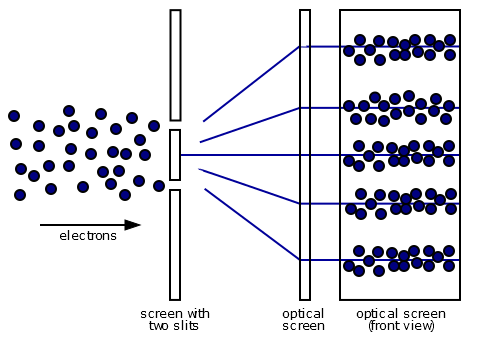
\includegraphics[width=.45\textwidth]{Two-Slit_Experiment_Electrons.png}}  ;
 \node[below right] at (interfere.south west) {(A) Particles exhibiting interference.};
 \node[inner sep=0pt] (noninterfere) at (7.7,0)
 {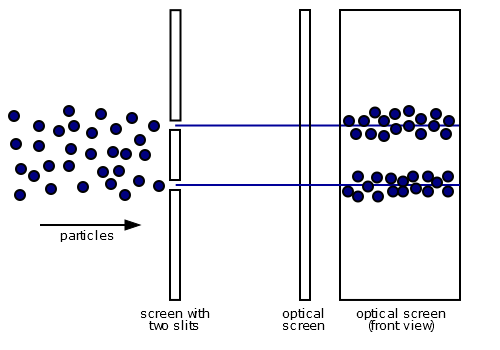
\includegraphics[width=.45\textwidth]{Two-Slit_Experiment_Particles.png}};
 \node[below right] at (noninterfere.south west) {(B) Particles not exhibiting interference.};
\end{tikzpicture}
\vspace*{10px}
\caption{The Double-Slit Experiment. Particles are incident on a double slit. In diagram (A), the particles are exhibiting an interference pattern, whereas in diagram (B), the particles are not exhibiting an interference pattern. Whether or not there is interference will depend on factors such as the size of the particles and whether it can be ascertained which slit the particle went through. The larger the particles are or the more information available as to which slit the particle went through, the less likely the particles will exhibit interference.\protect\footnotemark}
\label{DoubleSlit}
\end{figure}
As figure \ref{DoubleSlit} indicates, when a beam of particles is incident on a double slit, the particles that are detected on the detection screen are distributed according to a distribution pattern which either exhibits quantum interference as shown on the left in the figure, or does not exhibit such interference as shown on the right. Small particles like electrons and photons will tend to exhibit quantum interference, whereas mesoscopic particles  will not typically exhibit quantum interference. 

To explain what is going on, we suppose that when just the top slit is open, the normalized state of the particle is $\ket{\psi_1}$,\label{psi_slit} whereas if just the bottom slit is open, we suppose that the normalized state of the particle is $\ket{\psi_2}$, and when both slits are open, we suppose that the state of the particle will be $\frac{1}{\sqrt{2}}(\ket{\psi_1}+\ket{\psi_2})$. 
 Now let the variable $x$ describe the position on the detection screen. For instance, we might take $x=0$ to be the center of the detection screen, and take  positive values of $x$ as corresponding to positions on the upper part of the screen, and negative values of $x$ as corresponding to positions on the lower part of the screen, but the precise convention we adopt won't matter.\footnotetext{Diagrams (A) and (B) are by inductiveload, and are Public domain, via Wikimedia Commons. Sources: https://commons.wikimedia.org/wiki/File:Two-Slit\_Experiment\_Electrons.svg and https://commons.wikimedia.org/wiki/File:Two-Slit\_Experiment\_Particles.svg.} Then we define the  $\ket{x}$-state\footnotemark\;as the physical state describing the particle to be exactly located at position $x$ on the screen. Note that the state $\ket{x}$ is indexed by a continuous parameter, $x$. This is in contrast to the basis of states $\ket{s_i}$ which we have been considering up until now which are indexed by discrete values of $i$ such as $i=1,\,2,\ldots.$ Because of this difference, we need to use calculus to deal with $\ket{x}$-states in a rigorous manner, but such details will not concern us here. In reality, because of the Heisenberg uncertainty principle, a particle is never in just one $\ket{x}$-state, but rather the particle will be in a superposition of many $\ket{x}$-states, which may or may not be concentrated around a particular location, $x_0$ say. The more concentrated these  $\ket{x}$-states of this superposition are concentrated around a particular location $x_0$, the more the particle will have the particle-like characteristic of being localized in one place. But if the  $\ket{x}$-states of this superposition are more spread out, the particle will have more wave-like characteristics. So when physicists speak of particles, often they are not thinking of physical entities that are very localized in position, as non-physicists would think. Nevertheless, at the moment the particle is detected on the detection screen, it does seem to be highly localized.\footnotetext{$\ket{x}$ is not really a state in the proper sense. With the states we've seen so far, when $\ket{\phi}$ and $\ket{\psi}$ have been normalized, then $\abs{\ip{\phi}{\psi}}^2$ will be a conditional probability, and hence at most $1$. However, $\ket{x}$ cannot be normalized. This is because the bracket  $\ip{x}{y}$ is defined to be $\ip{x}{y}=\var(x-y)$ where $\var(x)$ is the Dirac delta function such that \begin{equation} 
\var(x)=
\begin{cases} \infty & \text{if $x=0$,} \\
0 & \text{if $x\neq 0$}.
\end{cases}
\end{equation} and has the property that 
$\int \dd x \var(x) f(x) = f(0)$ for any continuous function $f(x)$. The theory of distributions allows one to deal rigorously with Dirac delta functions. E.g. see \cite[ch. 6]{Rudin}.  
}

 Given a state $\ket{\psi}$ for a so-called particle, we define the function $\psi(x)=\ip{x}{\psi}$. Because of the continuous nature of the variable $x$ (in contrast to the discrete nature of $i$ in a basis $\{\ket{s_i}:i\}$), the function $\rho(x)=\abs{\psi(x)}^2\label{rhodensity}$ determines a probability density for a range of outcomes rather than a probability for a specific outcome. Here, we do not need to go into the details of probability densities,\footnote{But if you are interested, a probability density $\rho(x)$ for a random variable $X$ that has real values is a function such that $\rho(x)\geq 0\, \,\forall x\in\mathbb{R}$, and that $\int_\mathbb{R} \rho(x) \dd x =1$ and the probability that $X$ has a value in the subset $U\subset\mathbb{R}$ is $\int_U \rho(x) \dd x $. } but roughly speaking, the greater the value of $\rho(x)$, the greater will be the relative probability of detecting the particle at location $x$. Thus, if $\rho(x)=0$, then the particle would not be detected at location $x$. 

Now if  $\ket{\psi}=\frac{1}{\sqrt{2}}(\ket{\psi_1}+\ket{\psi_2})$, then 
$\psi(x)=\frac{1}{\sqrt{2}}(\psi_1(x)+\psi_2(x)).$ Therefore, the corresponding probability density will be
\begin{equation*}\abs{\psi(x)}^2=\frac{1}{2}(\abs{\psi_1(x)}^2+\abs{\psi_2(x)}^2+2\Re(\overline{\psi_1(x)}\psi_2(x)).\protect\footnotemark
\end{equation*}
\footnotetext{Here $\Re$ means the real part of a complex number. Thus if the complex number $z=\alpha+i\beta$ for real numbers $\alpha$ and $\beta$, then $\Re(z)=\alpha$. To see why the above equation holds, we recall that $\abs{z}^2=z\overline{z}$ and that $\Re(z)=\frac{1}{2}(z+\overline{z})$. Therefore if $z=\frac{1}{\sqrt{2}}(v+w)$ for complex number $v$ and $w$, then $\abs{z }^2 =\frac{1}{\sqrt{2}}(v+w)\frac{1}{\sqrt{2}}\overline{(v+w)}= \frac{1}{2}(v+w)\overline{(v+w)}=\frac{1}{2}(v\overline{v}+w\overline{w}+w\overline{v}+v\overline{w})=\frac{1}{2}(\abs{v}^2+\abs{w}^2+w\overline{v}+\overline{w\overline{v}})=\frac{1}{2}(\abs{v}^2+\abs{w}^2+2\Re(\overline{v}w))$.}Now when the detection screen is far away from the double slits, we will have $\abs{\psi_1(x)}^2\approx \abs{\psi_2(x)}^2$ for $x$ near the center point on the screen. However, depending on slight changes in the value of $x$ from the center point on the screen, sometimes $\psi_1(x)$ and $\psi_2(x)$ will be in phase so that  $\psi_1(x)\approx\psi_2(x)$, in which case $\abs{\psi(x)}^2\approx 2\abs{\psi_1(x)}^2$. But sometimes $\psi_1(x)$ and $\psi_2(x)$ will be  out of phase so that $\psi_1(x)\approx-\psi_2(x),$ in which case $\abs{\psi(x)}^2\approx 0$. Hence we get the interference pattern as shown in figure \ref{DoubleSlit} (A).

Now in order to consider how decoherence affects interference, we let $$\ket{\Psi(t)}=\frac{1}{\sqrt{2}}(\ket{\psi_1}\ket{E_1(t)}+\ket{\psi_2}\ket{E_2(t)})$$ be the state of the composite system $\mathcal{U}=\mathcal{S}+\mathcal{E}$ where $\mathcal{S}$ is a particle that has gone through the double slit and will be detected on the detection screen, and $\mathcal{E}$ is the local environment of the experimental set up. The expression for $\ket{\Psi(t)}$ indicates that we are assuming  $\mathcal{S}$ doesn't become entangled with $\mathcal{E}$ when $\mathcal{S}$ is in the state $\ket{\psi_1}$ or $\ket{\psi_2}$. Corresponding to $\ket{\Psi(t)}$ we can define the density matrix  $\hat{\rho}(t)=\dyad{\Psi(t)}.$  We can also define the observable\footnote{Note that we only call $\dyad{x}_\mathcal{S}$ an observable in an analogical sense since it is not a compact Hermitian operator acting on the Hilbert space of states $H_\mathcal{S}$. If we were being more rigorous, we would need to consider a Hermitian operator of the form $\int \sigma(x)\dyad{x}_\mathcal{S}\dd x$ for an appropriate test function $\sigma(x)$. } $\dyad{x}_\mathcal{S}$ for the system $\mathcal{S}$ so that $\dyad{x}_\mathcal{S}\ket{\psi}_\mathcal{S}=\psi(x)\ket{x}_\mathcal{S}.$ As we saw in equation (\ref{extension}) on page \pageref{extension}, we can naturally extend the action of $\dyad{x}_\mathcal{S}$ to $H_\mathcal{U}$.\footnote{Strictly speaking, it is not $\dyad{x}_\mathcal{S}$ that is extended to act on $H_\mathcal{U}$, but rather a Hermitian operator of the form $\int \sigma(x)\dyad{x}_\mathcal{S}\dd x$ for an appropriate test function $\sigma(x)$ that is extended to $H_\mathcal{U}$. For a state $\ket{\xi}_\mathcal{U}=\ket{\psi}_\mathcal{S}\ket{E}_\mathcal{E}$, the action of $\dyad{x}_\mathcal{U}$ on $\ket{\xi}_\mathcal{U}$ gives the `state' $\dyad{x}_\mathcal{U}\ket{\xi}_\mathcal{U}\myeq\psi(x)\ket{x}_\mathcal{S}\ket{E}_\mathcal{E}$, but since this is not normalizable, we have to `smear' it by integrating it with respect to the test function $\sigma(x)$.}  
This allows us to define 
$$\rho_\mathcal{U}(x, t)\myeq\Tr_\mathcal{U}(\hat{\rho}(t)_\mathcal{U}\dyad{x}_\mathcal{U}).$$
 In the specific case when $\hat{\rho}_\mathcal{U}(t)=\dyad{\xi(t)}_\mathcal{U}$ where $\ket{\xi(t)}_\mathcal{U}=\ket{\psi}_\mathcal{S}\ket{E(t)}_\mathcal{E}$ for normalized states $\ket{\psi}_\mathcal{S}$ and $\ket{E(t)}_\mathcal{E}$, we have $\rho_\mathcal{U}(x, t) =\abs{\psi(x)}^2$ which is equal to the probability density function $\rho(x)$ we saw on page \pageref{rhodensity}.\footnote{To see this, note that we can ignore $\mathcal{E}$ in calculating $\ev*{\dyad{x}_\mathcal{U}}_\xi$ since when $\mathcal{S}$ and $\mathcal{E}$ are not entangled, $\ev*{\dyad{x}_\mathcal{U}}_\xi = \ev*{\dyad{x}_\mathcal{S}}_\psi$ as explained in footnote \ref{untangledobservable}. We can therefore just consider $\mathcal{S}$ and drop the subscripts.
Furthermore, as we saw on page \pageref{traceev}, $\ev*{\hat{\Lambda}}_\psi=\Tr(\hat{\rho}\hat{\Lambda})$ where $\hat{\rho}=\dyad{\psi}$. 
We can thus take an orthonormal basis $\{\ket{\psi_1},\ket{\psi_2},\ldots\}$ of $H_\mathcal{S}$ with $\ket{\psi_1}=\ket{\psi}$. 
Then $\rho(x)=\Tr(\hat{\rho}\dyad{x})=\Tr(\dyad{\psi}\dyad{x})=\sum_i\ip{\psi_i}{\psi}\ip{\psi}{x}\ip{x}{\psi_i}=\ip{\psi_1}{\psi}\ip{\psi}{x}\ip{x}{\psi_1} =\ip{\psi}{x}\ip{x}{\psi}=\overline{\ip{x}{\psi}}\ip{x}{\psi}=\abs{\ip{x}{\psi}}^2=\abs{\psi(x)}^2.$} 
However, if $\ket{E_1(t)}_\mathcal{E}$ is not proportional to $\ket{E_2(t)}_\mathcal{E}$, then $\ket{\Psi(t)}$ will be an entangled state of $\mathcal{S}$ and $\mathcal{E}$. But whether or not $\mathcal{S}$ and $\mathcal{E}$ are entangled, we can still use equation (\ref{reduced}) to calculate the partial trace:
$$\hat{\rho}_\mathcal{S}(t)=\frac{1}{2}(\dyad{\psi_1}_\mathcal{S}+\dyad{\psi_2}_\mathcal{S}+\ip{E_2(t)}{E_1(t)}_\mathcal{E} \dyad{\psi_1}{\psi_2}_\mathcal{S}+\ip{E_1(t)}{E_2(t)}_\mathcal{E} \dyad{\psi_2}{\psi_1}_\mathcal{S}).$$
By equation (\ref{reducedev}), we therefore have
\begin{equation}\rho_\mathcal{U}(x, t)=\frac{1}{2}\Big(\abs{\psi_1(x)}^2+\abs{\psi_2(x)}^2+2\Re\big(\ip{E_2(t)}{E_1(t)}_\mathcal{E}\overline{\psi_2(x)}\psi_1(x)\big)\Big).\protect\footnotemark
\end{equation}
Thus, \footnotetext{The calculation is as follows
  \begin{equation*}
\begin{split}\rho_\mathcal{U}(x, t)&=\Tr_\mathcal{U}(\hat{\rho}(t)_\mathcal{U}\dyad{x}_\mathcal{U})=
\ev*{\dyad{x}_\mathcal{U}}_{\rho(t)}=\Tr_\mathcal{S}(\hat{\rho}_\mathcal{S}(t)\dyad{x}_\mathcal{S})\\
&=\Tr_\mathcal{S}\Big(\frac{1}{2}(\dyad{\psi_1}_\mathcal{S}+\dyad{\psi_2}_\mathcal{S}+\ip{E_2(t)}{E_1(t)}_\mathcal{E} \dyad{\psi_1}{\psi_2}_\mathcal{S}+\ip{E_1(t)}{E_2(t)}_\mathcal{E} \dyad{\psi_2}{\psi_1}_\mathcal{S})\dyad{x}_\mathcal{S}\Big)\\
&=\Tr_\mathcal{S}\Big(\frac{1}{2}(\ip{\psi_1}{x}_\mathcal{S}\dyad{\psi_1}{x}_\mathcal{S}+\ip{\psi_2}{x}_\mathcal{S}\dyad{\psi_2}{x}_\mathcal{S}\\&\qquad+\ip{E_2(t)}{E_1(t)}_\mathcal{E}\ip{\psi_2}{x}_\mathcal{S}\dyad{\psi_1}{x}_\mathcal{S}+\ip{E_1(t)}{E_2(t)}_\mathcal{E} \ip{\psi_1}{x}_\mathcal{S}\dyad{\psi_2}{x}_\mathcal{S})\Big)
\\
&=\frac{1}{2}\Big(\ip{\psi_1}{x}_\mathcal{S}\ip{x}{\psi_1}_\mathcal{S}+\ip{\psi_2}{x}_\mathcal{S}\ip{x}{\psi_2}_\mathcal{S}\\&\qquad+\ip{E_2(t)}{E_1(t)}_\mathcal{E}\ip{\psi_2}{x}_\mathcal{S}\ip{x}{\psi_1}_\mathcal{S}+\ip{E_1(t)}{E_2(t)}_\mathcal{E}\ip{\psi_1}{x}_\mathcal{S}\ip{x}{\psi_2}_\mathcal{S}\Big)\\
&=\frac{1}{2}\Big(\overline{\ip{x}{\psi_1}_\mathcal{S}}\ip{x}{\psi_1}_\mathcal{S}+\overline{\ip{x}{\psi_2}_\mathcal{S}}\ip{x}{\psi_2}_\mathcal{S}\\&\qquad+\ip{E_2(t)}{E_1(t)}_\mathcal{E}\overline{\ip{x}{\psi_2}_\mathcal{S}}\ip{x}{\psi_1}_\mathcal{S}+\overline{\ip{E_2(t)}{E_1(t)}_\mathcal{E}\overline{\ip{x}{\psi_2}_\mathcal{S}}\ip{x}{\psi_1}_\mathcal{S}}\Big)
\\
&=\frac{1}{2}\Big(\abs{\psi_1(x)}^2+\abs{\psi_2(x)}^2+2\Re\big(\ip{E_2(t)}{E_1(t)}_\mathcal{E}\overline{\psi_2(x)}\psi_1(x)\big)\Big).
\end{split}
\end{equation*}}if $\ip{E_1(t)}{E_2(t)}_\mathcal{E}\approx 0$ then 
$\rho_\mathcal{U}(x, t)\approx\frac{1}{2}\Big(\abs{\psi_1(x)}^2+\abs{\psi_2(x)}^2\Big)$
and so we would observe a distribution pattern not exhibiting interference  as shown in figure \ref{DoubleSlit} (B), whereas if  $\ip{E_1(t)}{E_2(t)}_\mathcal{E}\not\approx 0$ we would get a distribution pattern exhibiting interference as shown in figure \ref{DoubleSlit} (B). Thus, decoherence theory gives us a means of determining whether or not quantum interference will be exhibited. 

\section{The Problem of Outcomes}\label{probOutcomes}
In the last two sections we have seen how decoherence theory solves the preferred basis problem and the problem of the nonobservability of interference. However, there is a third fundamental problem in quantum physics which decoherence theory is unable to solve. This is the problem of outcomes. As discussed in subsection \ref{vonNeumannMeasurement}, in the von Neumann measurement scheme, it is supposed that for the measurement of a physical system $\mathcal{S}$ to take place, it must interact with a measuring device $\mathcal{A}$ which together satisfy the conditions 1. and 2. on page \pageref{vonNeumannMeasurement1}. If $\mathcal{S}$ is initially in a superposition of states $\ket{\psi}=\sum_i c_i\ket{s_i}$ then for $\mathcal{A}$ to measure $\mathcal{S}$, it is necessary for the combined system $\mathcal{S}+\mathcal{A}$ to enter into a superposition
\begin{equation}\label{vNevolution}
\ket{\psi}\ket{a_r(t_0)}\xrightarrow{\text{time evolution}}\sum_i c_i\ket{s_i}\ket{a_i(t)}.
\end{equation}
However, although the evolution described in (\ref{vNevolution}) must take place if $\mathcal{A}$ is to measure $\mathcal{S}$, it is not sufficient. When one takes the partial trace of $\dyad{\psi}$ over $\mathcal{A}$, then according to (\ref{reduced}),
\begin{equation}\label{vNevolution2}
\tr_\mathcal{A}(\dyad{\psi})\xrightarrow{\text{time evolution}}\sum_i \abs{c_i}^2\dyad{s_i}.
\end{equation}
But as noted on page \pageref{Espagnat}, we cannot give an ignorance interpretation to $\sum_i c_i\dyad{s_i}$ for as d'Espagnat puts it, this is an improper mixture. When considered together, the system $\mathcal{S}$ and the apparatus $\mathcal{A}$ remain in the superposition described by (\ref{vNevolution}), and so none of the measurement outcomes from the set of possible outcomes $\{\ket{s_i}\}$ have actually occurred. The problem of explaining how the composite system   $\mathcal{S}+\mathcal{A}$       goes from being in the state $\sum_i c_i\ket{s_i}\ket{a_i(t)}$ to a state $\ket{s_i}\ket{a_i(t)}$ is known as the \textbf{problem of outcomes}. 


\section{The Many-Worlds Interpretation}\label{manyworldsinterpretation1}
Not everyone is convinced that the problem of outcomes is a genuine problem. In particular, people who endorse the many-worlds interpretation of quantum physics effectively argue that there are no outcomes in the traditional sense. In this section, we now give and account of the many-worlds interpretation of quantum physics and why physicists find it attractive. To this end, let us consider a physical universe $\mathcal{U}=\mathcal{S}+\mathcal{A}+\mathcal{P}_A+\mathcal{P}_B+\mathcal{E}$ consisting of subsystems $\mathcal{S}, \mathcal{A}, \mathcal{P}_A,\mathcal{P}_B$ and $\mathcal{E}$. $\mathcal{S}$ is the physical system under investigation; $\mathcal{A}$ is some measuring apparatus that interacts with $\mathcal{S}$; $\mathcal{P}_A$ and $\mathcal{P}_B$ are the physical systems corresponding to two scientists, Alice and Bob who observed the apparatus $\mathcal{A}$; and $\mathcal{E}$ is the remainder of the physical universe $\mathcal{U}$.  For convenience, we define the composite subsystem $\mathcal{V}=\mathcal{S}+\mathcal{A}+\mathcal{P}_A+\mathcal{P}_B$ so that $\mathcal{U}=\mathcal{V}+\mathcal{E}$. As above on page \pageref{pointer}, we  assume that there is an orthonormal basis $\{\ket{s_i}:i\}$ of $H_\mathcal{S}$ which we again refer to as pointer states, but now we assume that there are ready states $\ket{a_r(t)}\in H_\mathcal{A},\,\ket{p_{r, A}(t)}\in H_{\mathcal{P}_A},\,\ket{p_{r, B}(t)}\in H_{\mathcal{P}_B},$ and $\ket{E_r(t)}\in H_\mathcal{E}$ and that for each $i$, there are normalized states $\ket{a_i(t)}\in H_\mathcal{A},\,\ket{p_{i, A}(t)}\in H_{\mathcal{P}_A},\,\ket{p_{i, B}(t)}\in H_{\mathcal{P}_B},$ and $\ket{E_i(t)}\in H_\mathcal{E}$ such that 
\begin{enumerate}[noitemsep, nosep, topsep=0pt]
\item for any $t\geq 0$ we have the evolution of the states 
\begin{align*}\ket{s_i}\ket{a_r(t)}\ket{p_{r, A}(t)}&\ket{p_{r, B}(t)}\ket{E_r(t)}\\ &\xrightarrow{\text{time evolution}}\ket{s_i}\ket{a_i(t)}\ket{p_{i, A}(t)}\ket{p_{i, B}(t)}\ket{E_i(t)},\end{align*}
\item there exists $\delta>0$ such that if $t>t_0+\delta$, then for $i\neq j$, $\ip{a_i(t)}{a_j(t)}\approx 0$, $\ip{p_{i, A}(t)}{p_{j, A}(t)}\approx 0$, $\ip{p_{i, B}(t)}{p_{j, B}(t)}\approx 0$ and $\ip{E_i(t)}{E_j(t)}\approx 0$.\footnote{Again, recall footnote \ref{approx}.}
\end{enumerate}
We also suppose that the $\ket{p_{i,A}(t)}$-state would describe actions of Alice consistent with her observing the apparatus being in the $\ket{a_i(t)}$-state, for example, her writing down in her log book that the apparatus is in the $\ket{a_i(t)}$-state or telling her colleague that this is the case. Likewise, we assume the $\ket{p_{i,B}(t)}$-state is consistent with Bob also observing the apparatus to be in the $\ket{a_i(t)}$-state.

Now suppose the initial (normalized) state of $\mathcal{S}$ is $\ket{\psi}=\sum_i c_i\ket{s_i}$, so that the state for the composite system $\mathcal{U}$ is $\ket{\Psi(t)}=\sum_i c_i \ket{\xi_i(t)}\ket{E_i(t)}$ where $\ket{\xi_i(t)}=\ket{s_i}\ket{a_i(t)}\ket{p_{i,A}(t)}\ket{p_{i,B}(t)}$. We also define the corresponding density matrix for the composite system $\hat{\rho}=\dyad{\Psi}$. If we were unable to make any observations on $\mathcal{E}$, then 
 the partial trace
$\hat{\rho}_{\mathcal{V}}(t)=\Tr_\mathcal{E}(\hat{\rho}(t))$ will contain all the information we need to work out the expectation values for any observables of  $\mathcal{V}.$ So just as with equation (\ref{reduced}), we will have
\begin{equation} \label{reducedv}
\begin{split}
  \hat{\rho}_{\mathcal{V}}(t)&=\sum_{i}\abs{c_i}^2\dyad{\xi_i(t)}+\sum_{i\neq j}c_i\overline{c_j}\ip{E_j(t)}{E_i(t)}\dyad{\xi_i(t)}{\xi_j(t)}\\
  &\approx \sum_{i}\abs{c_i}^2\dyad{\xi_i(t)}
  \end{split}\end{equation}
  for $t>t_0+\delta.$ Then the expectation values of any observables on $\mathcal{V}$ will be indistinguishable from the scenario in which $\mathcal{V}$ is actually in one of the $\ket{\xi_i(t)}$-states with probability $\abs{c_i}^2$.\footnote{Again recall the discussion following equation (\ref{rhodiag}) on page \pageref{rhodiag}. There is the question of uniqueness of $\hat{\rho}_{\mathcal{V}}=\sum_{i}\abs{c_i}^2\dyad{\xi_i(t)}$. If all the $\abs{c_i}^2$ are unique, then if we have another decomposition $\hat{\rho}_{\mathcal{S}+\mathcal{A}+\mathcal{P}_A+\mathcal{P}_B}=\sum_{i}\abs{c_i}^2\dyad{\xi_i'(t)}$ it follows that $\ket{\xi_i(t)}\propto\ket{\xi_i'(t)}$. But even if some of the $\abs{c_i}^2$ are the same, criteria 1 and 2 above will ensure that states with the same  value of $\abs{c_i}^2$ will be determined up to permutation.} It would nevertheless be incorrect for us to conclude on the basis of decoherence theory alone that $\mathcal{V}$ actually was in one of those $\ket{\xi_i(t)}$-states, since equation (\ref{reducedv}) is based on a subjective distinction between $\mathcal{V}$ and $\mathcal{E}$ in the decomposition $\mathcal{U}=\mathcal{V}+\mathcal{E}.$ Human scientists make this distinction to reflect the fact that they can only perform measurements on $\mathcal{V}$ and can't measure $\mathcal{E}$. But if a super-intelligent being could measure everything in  $\mathcal{U}$, then such a being would not say that $\mathcal{V}$ was in one of the  $\ket{\xi_i(t)}$-states, but rather that $\mathcal{U}$ was in the state $\ket{\Psi(t)}$. As we have already discussed on pages \pageref{subtle}--\pageref{subtleend}, the density matrix $ \hat{\rho}_{\mathcal{V}}(t)$ is not a mixed state, but is an improper mixture. 

Now if we define the observables $\hat{\Lambda}_{i,\mathcal{A}}(t)=\dyad{p_{i,A}(t)}$ that would measure the behavior of Alice, and the observables $\hat{\Lambda}_{i,\mathcal{B}}(t)=\dyad{p_{i,B}(t)}$ that would measure the behavior of Bob, then for $t>t_0+\delta$, we see that $\hat{\Lambda}_{i,\mathcal{A}}(t)\hat{\Lambda}_{j,\mathcal{B}}(t)\ket{\Psi(t)}\approx 0,$ when $i\neq j$. This means that when we consider $\hat{\Lambda}_{i,\mathcal{A}}(t)\hat{\Lambda}_{j,\mathcal{B}}(t)$ as an observable acting on $\mathcal{V}$,  the expectation value $\ev*{\hat{\Lambda}_{i,\mathcal{A}}(t)\hat{\Lambda}_{j,\mathcal{B}}(t)}_{\rho_\mathcal{V}(t)}$ will be approximately zero for $i\neq j$. What this means is that if we consider ourselves as observing Alice and Bob observing the apparatus, then after time $t_0+\delta$, the probability we would see Alice and Bob disagreeing with each other concerning their observations of the apparatus would be approximately 0. 
 On the other hand, since $\hat{\Lambda}_{i,\mathcal{A}}(t)\hat{\Lambda}_{i,\mathcal{B}}(t)\ket{\Psi(t)} \approx c_i \ket{\xi_i(t)}\ket{E_i(t)}$ for $t>t_0+\delta$, it follows that $\ev*{\hat{\Lambda}_{i,\mathcal{A}}(t)\hat{\Lambda}_{i,\mathcal{B}}(t)}_{\rho_\mathcal{V}(t)}=\abs{c_i}^2.$ 
 We would thus observe Alice and Bob observing the apparatus to be in the $\ket{a_i(t)}$-state with probability $\abs{c_i}^2.$ 
 
 But note that on the assumption that there are no hidden variables, if we did actually make such an observation and this observation corresponded to reality, then the quantum state $\ket{\Psi(t)}$ would have had to have changed to $\ket{\xi_i(t)}\ket{E_i(t)}$, since before our observation when $\ket{\Psi(t)}$ was a complete description of $\mathcal{U}$, we would say Alice and Bob will measure the $\ket{a_i(t)}$-state with probability $\abs{c_i}^2$, but when we are actually seeing them measuring the $\ket{a_i(t)}$-state, we would have to say that now the probability they are measuring the $\ket{a_i(t)}$-state is $1$, and hence we would say that the system was in the $\ket{\xi_i(t)}\ket{E_i(t)}$-state. Whether or not the process of the state going from $\ket{\Psi(t)}$ to $\ket{\xi_i(t)}\ket{E_i(t)}$ was instantaneous or took a non-infinitesimal amount of time, this interpretation would be susceptible to the problems already discussed with the Copenhagen interpretation on page \pageref{Copenhagenproblem}.

But in the \textbf{many-worlds interpretation}, rather than assuming that $\ket{\Psi(t)}=\sum_i c_i \ket{\xi_i(t)}\ket{E_i(t)}$ is the complete description of $\mathcal{U}$ that enables us to work the probability of certain outcomes, we simply say that $\ket{\Psi(t)}$ is a complete description of the state of $\mathcal{U}$, and we drop the assumption that we need to interpret this state as describing probabilities of outcomes. Thus a many-worlds adherent would say we can understand what the state of $\mathcal{U}$ is on its own terms without the need to appeal to any other extrinsic principle such as measurement. Just as we don't puzzle over how to interpret what a sphere is in terms of an extrinsic principle, we don't need to puzzle over how to interpret the states of $\mathcal{U}$. We can think of the mathematical formalism $\ket{\Psi(t)}=\sum_i c_i \ket{\xi_i(t)}\ket{E_i(t)}$ describing the state of $\mathcal{U}$ as being somewhat akin to the equation $x^2+y^2+z^2=1$ describing a sphere. Although we might be tempted to interpret $\ket{\Psi(t)}$ as describing the probability of outcomes, we are not obliged to do so,  since these probabilities can instead be understood to be grounded in the symmetries the system possesses rather than in terms of the frequency of how many measurement outcomes are likely to occur. For instance, when we see a coin and judge that it will come up heads with probability $\frac{1}{2}$ and tails with probability $\frac{1}{2}$, we intuit this by looking at the symmetry of the coin rather than tossing the coin millions of times and counting how often it comes up heads and how often it comes up tails.
 
As for the decomposition $\ket{\Psi(t)}=\sum_i c_i \ket{\xi_i(t)}\ket{E_i(t)}$  in terms of the $\ket{\xi_i(t)}\ket{E_i(t)}$ basis states, decoherence theory gives us a natural account of why we should choose this basis rather than any other. When $\mathcal{U}$ is in the state $\ket{\Psi(t_0)}=\Big(\sum_i c_i \ket{\xi_i(t_0)}\Big)\ket{E_r(t)}$, we can think of this state as describing one world, $W$ say. But once $t>t_0+\delta$ so that $\ip{E_i(t)}{E_j(t)}\approx 0$ for $i\neq j$, we can think of each $\ket{\xi_i(t)}\ket{E_i(t)}$-component as a different world $W_i$. Thus, for $t>t_0+\delta$, we say the world $W$ has \textbf{branched} into as many-worlds $W_i$ for which the $c_i$ are non-zero. 

But why should we think that there are literally many worlds? Well, from an ontological point of view, one might very well think that there is really only one world and that this world is described by $\ket{\Psi(t)};$ it would be a rather weird world since the entanglement between $\mathcal{V}$ and $\mathcal{E}$ would mean there wouldn't be any absolute matters of fact describing $\mathcal{V}$. But it might not be a bad thing to say that the ``many'' in the many-worlds interpretation is really just a figure of speech that we shouldn't take too literally, since a common objection to the many-worlds interpretation is that it is ontologically extravagant and that we should appeal to Occam's Razor. However, if we just say that there is actually only one world described by $\ket{\Psi(t)}$ then this ``many''-worlds interpretation is actually rather parsimonious from an ontological point of view. 

But if by literal, we mean descriptive rather than ontological, it does seem rather natural to say that there are literally many worlds. For although we might initially suspect that the worlds $W_i$ and $W_j$ are not well-defined given the fact that $\ip{E_i(t)}{E_j(t)}$ is very small but not zero for $i\neq j$, we can nevertheless expect $\ip{\xi_i(t)}{\xi_j(t)}$ to be identically zero for $i\neq j$, just as we can expect $\ip*{\uvbp{a}}{\uvbm{a}}$ to be identically zero.\footnote{It is also reasonable to suppose that in situations such as the double-slit experiment described on page \pageref{psi_slit} that $\ip{\psi_1(t)}{\psi_2(t)}$ is identically zero. This is because $\ip{\psi_1(t)}{\psi_2(t)}$ when $t$ is the time at which the particle is going through the slit, and this will remain zero because of a property of the time evolution operator known as unitarity.} Thus, if we define $\ket{W_i(t)}=\ket{\xi_i(t)}\ket{E_i(t)},$ then the $\ip{W_i(t)}{W_j(t)}$ will be identically zero for $i\neq j$. 

Still, the supposition that $\ket{\Psi(t)}= \sum_i c_i\ket{W_i(t)}$  with $\ip{W_i}{W_j}=0$ for $i\neq j$ is not of itself sufficient justification for describing the state $\ket{\Psi(t)}$ as a composition of mutually exclusive world descriptions given by the $\ket{W_i(t)}$. After all, the fact that
\begin{align*}\ket{\text{Cat Alive}}= &\frac{1}{\sqrt{2}}\Big(\frac{1}{\sqrt{2}}(\ket{\text{Cat Alive}}+\ket{\text{Cat Dead}})\Big)\\&+\frac{1}{\sqrt{2}}\Big( \frac{1}{\sqrt{2}}(\ket{\text{Cat Alive}}-\ket{\text{Cat Dead}})\Big). \end{align*} does not incline us to think of the state $\ket{\text{Cat Alive}}$ as being composed of the mutually exclusive cat states  $\frac{1}{\sqrt{2}}(\ket{\text{Cat Alive}}+\ket{\text{Cat Dead}})$ and $\frac{1}{\sqrt{2}}(\ket{\text{Cat Alive}}-\ket{\text{Cat Dead}})$. 

The key justification for describing the state $\ket{\Psi(t)}$ as a composition of the mutually exclusive $\ket{W_i(t)}$-states is the fact that the states $\ket{\xi_i(t)}$ and $\ket{\xi_j(t)}$ decohere for $i\neq j$, that is, the off-diagonal entries $\dyad{\xi_i(t)}{\xi_j(t)}$ of the reduced density matrix $\hat{\rho}_\mathcal{V}(t)$ will tend to zero, and as we saw in section \ref{Nonobservability}, it will follow that quantum interference effects between $\ket{\xi_i(t)}$ and $\ket{\xi_j(t)}$ will then tend to zero. Thus, when it comes to observables defined on $\mathcal{V}$, using equations (\ref{reducedev}) and (\ref{reducedv}), we can calculate the expectation value of an observable $\hat{\Lambda}_\mathcal{V}$  as a weighted sum of expectation values for each of the states $\ket{\xi_i(t)}$:
\begin{equation}\label{manyapprox}\ev*{\hat{\Lambda}_\mathcal{U}}_{\Psi(t)}\approx\sum_i |c_i|^2 \ev*{\hat{\Lambda}_\mathcal{V}}_{\xi_i(t)}.\end{equation}
The fact that (\ref{manyapprox}) is only an approximation suggests that the time at which branching occurs is not well-defined. All that we can do is choose a time sufficiently large $\delta$ so that for  $t>t_0+\delta$, the approximation (\ref{manyapprox}) meets our desired level of accuracy. 

Despite this vagueness on when branching occurs, we can still form a natural and well-defined notion of worlds according to the following definition: \label{rigorousworld} a set $\{W_i: i\}$ is the set of worlds for a universe $\mathcal{U}=\mathcal{V}+\mathcal{E}$ when 
 \begin{enumerate}[noitemsep, nosep, topsep=0pt]
 \item $W_i$ is a description of $\mathcal{U}$ given by $\ket{W_i(t)}=\ket{\xi_i(t)}\ket{E_i(t)}$,
 \item $\mathcal{U}$ is in the state $\ket{\Psi(t)}=\sum_i c_i \ket{W_i(t)}$ with all $c_i\neq 0$.
 \item $\ip{\xi_i(t)}{\xi_j(t)}=0$ for $i\neq j$,
 \item $\ip{E_i(t)}{E_j(t)}\rightarrow 0$ as $t\rightarrow\infty$ for $i\neq j$ and the convergence is such that for any observable $\hat{\Lambda}_\mathcal{V}$ defined on $\mathcal{V}$, $\ev*{\hat{\Lambda}_\mathcal{U}}_{\Psi(t)}\rightarrow\sum_i |c_i|^2 \ev*{\hat{\Lambda}_\mathcal{V}}_{\xi_i(t)}$. 
 \end{enumerate}
Note that according to this definition, the description $\ket{\Psi(t)}$ is rather trivially a world -- we just take the environment $\mathcal{E}$ to be empty so that there would be only one $\ket{E_i(t)}$ which would be the vacuum state. So there is at least one world according to this definition. There is a question of whether there could be more than one world and this would depend on whether we could really have a non-trivial decomposition $\mathcal{U}=\mathcal{V}+\mathcal{E}$, 
for the supposition that there is such a decomposition requires that it is possible to distinguish $\mathcal{V}$ and $\mathcal{E}$, but this might not in fact be possible. For instance, if the ultimate fate of the universe was that it would collapse into a singularity, then there would come a point at which it wouldn't be possible to make a distinction between $\mathcal{V}$ and $\mathcal{E}$. But despite this possible concern, the above definition makes it seem plausible that there could be many well-defined worlds $W_i$.\footnote{Recall that the purpose of this chapter is only to show why physicists might find the many-worlds interpretation of quantum physics attractive. It is not the purpose of this chapter to show that the many-worlds interpretation is without any problems. }

When we look at a particular $\ket{\xi_i(t)}$ it will look like it is describing a fairly classical world with scientists performing their measurements and agreeing about what they measure. And as long as the $\ket{\xi_i(t)}$-states remain pointer states with respect to $\ket{E_i(t)}$ no branching will occur. But typically, a $\ket{\xi_i(t)}$-state will not indefinitely remain a pointer state with respect to $\ket{E_i(t)}$. We can think of how this happens with the Stern-Gerlach experiment. For if one Stern-Gerlach apparatus has its magnetic field orientated in the $\uvb{a}$-direction, then $\ket{\uvbp{a}}$ and $\ket{\uvbm{a}}$ will be pointer states for a silver atom in the vicinity of this apparatus. But if the same silver atom then travels onward to another Stern-Gerlach apparatus with its magnetic field now orientated in the $\uvb{b}$-direction, $\ket{\uvbp{a}}$ and $\ket{\uvbm{a}}$ will no longer be pointer states with respect to their environment, and so branching will occur. But this is not necessarily a problem for the definition of many-worlds given above on page \pageref{rigorousworld}, for when a $\ket{\xi_i(t)}$-state does not indefinitely remain a pointer state with respect to $\ket{E_i(t)}$, we can just rewrite $\ket{\xi_i(t)}$ as a sum of pointer states $\ket{\xi_{ij}(t)}$ and $\ket{E_i(t)}$  as a sum of their respective environments $\ket{E_{ij}(t)}$, and then $\ket{E_i(t)}$ will be like a ready state for the $\ket{E_{ij}(t)}$. Assuming we can do this so that the $\ket{\xi_ij(t)}$ are orthogonal to the $\ket{\xi_{i'j'}(t)}$ when $i'\neq i$ or $j'\neq j$, then we would still be able to have well-defined worlds according to the definition given above.


\section{Evaluating the Many-Worlds Interpretation}\label{manyworldsinterpretation2}
Given the above account of the many-worlds hypothesis of quantum physics, it does seem understandable why physicists would find it so attractive. Although we can't specify an exact moment at which branching occurs, the idea of branching and of there being many worlds itself is not particularly mysterious. This can all be explained in terms of the dynamics of the system and the environment, and decoherence theory allows us to understand why the interference effects that are the hallmark of quantum physics generally disappear on the macroscopic level. 

There are other advantages  of the many-worlds hypothesis besides these which we need not discuss here.\footnote{More details can be found in \cite{Schlosshauer} and \cite{joos2013decoherence}.} But for all the advantages of the many-worlds hypothesis, there is one fundamental problem, and that is its patent absurdity. It seems that we should be able to say whether a cat is alive or dead without having to say what state the rest of the universe is in. However, the many-worlds hypothesis suggests that for any subsystem of the universe, we will in general only be able to say what state it is in with respect to the state of the rest of the universe. For example, if the state $\mathcal{S}$ is the system constituting a cat-wise configuration of particles and $\mathcal{E}$ is the rest of the universe, then given that the composite system $\mathcal{U}=\mathcal{S}+\mathcal{E}$ is described by the state $$\ket{\Psi(t)}=\frac{1}{\sqrt{2}}\big(\ket{\text{Cat Alive}}_\mathcal{S}\ket{E_\text{Cat Alive}}_\mathcal{E}+\ket{\text{Cat Dead}}_\mathcal{S}\ket{E_\text{Cat Dead}}_\mathcal{E}\big),$$ then we are in no position to make an absolute matter of fact claim about the system $\mathcal{S}$ and say the cat is dead or the cat is alive. Rather we have to say with respect to the environment described by $\ket{E_\text{Cat Alive}}_\mathcal{E}$, the cat is alive, and with respect to the environment $\ket{E_\text{Cat Dead}}_\mathcal{E}$, the cat is dead. According to the many-worlds hypothesis, the branching into multiple worlds doesn't just occur in rare instances, such as in Schr\"{o}dinger's cat type experiments. On the contrary, branching is supposed to be happening all the time.  Now anyone who has a common sense understanding of science would say that science enables us to understand absolute matters of fact about subsystems of the universe and the principles that govern them. But if there really are no such matters of fact, then we have to abandon this common sense understanding of science. Intuitively, it also seems obvious that I can know I am alive without needing to know the state of the rest of the universe, but the many-worlds hypothesis does not allow me to make this absolute matter of fact claim. So from a common sense point of view, the many-worlds hypothesis really is absurd.

 Of course some hypotheses may initially seem absurd, but once the hypothesis has been fully explained, it can appear far more plausible. For instance, time dilation in Special Relativity might initially sound absurd to some people, but once one has a better grasp of Special Relativity and is open to the possibility that  systems moving close to the speed of light with respect to ourselves might have properties rather different to systems that move with much slower speeds, then Special Relativity doesn't seem absurd at all.  
 
 However, the many-worlds hypothesis as presented here is different in this regard since it is not hypothesizing about some extreme situation. It is hypothesizing about ordinary situations. And one can have a fairly good understanding of the many-worlds hypothesis and still find it absurd. Some people choose to embrace the absurdity and reject common sense. But throughout much of human history, when a hypothesis has entailed an absurd conclusion, reasonable people have usually thought it better to reject the hypothesis rather than embrace the absurdity. 
  
 But in rejecting a hypothesis as absurd, it doesn't mean that absolutely everything in the hypothesis needs to be rejected, for  a hypothesis might be formulated in terms of sub-hypotheses, some of which might be very plausible, in which case something of the original hypothesis might be salvageable. In the case of the many-worlds hypothesis, I believe it does have something that is salvageable, namely decoherence theory. In the next chapter I will consider Adrian Kent's one-world interpretation of quantum physics in which the basic ideas of decoherence theory remain intact.






\printbibliography
\end{document}


